\section{Experimental Analysis}
\label{sec:evaluation}
In this section, we present the evaluation results. All experiments are carried out on an Intel Xeon processor. Table~\ref{tab:specification} summarizes the detailed specification of the hardware and software used in our experiments.
\begin{table}[t]
\centering
\caption{Specification of our evaluation platform}
\label{tab:specification}
\resizebox{0.45\textwidth}{!}{%
\begin{tabular}{|l|l|}
\hline
Component               & Description                                \\ \hline
Processor               & Intel(R) Xeon(R) Gold 6338 CPU @ 2.00GHz   \\ \hline
L3 Cache Size           & 48MiB                                      \\ \hline
Memory                  & 1024GB DDR4 RAM                             \\ \hline
OS                      & Ubuntu 22.04.4 LTS                         \\ \hline
Kernel                  & Linux 5.15.0-100-generic                    \\ \hline
Compiler                & GCC 11.4.0 with -O3                        \\ \hline
\end{tabular}%
} 
\end{table}

% % \algorithmTable
% \subcompact
% \subsection{Algorithm Selection}
% \label{subsec:algorithmselection}
% In our comparative analysis, \algo is benchmarked against eight established \dsc algorithms, summarized in Table~\ref{tab:summary}. The selection of these algorithms is guided by two primary criteria: 1) they collectively represent a broad spectrum of design decisions across all four design aspects, as detailed in Table~\ref{tab:summary}; 2) they span a historical range in the field, from foundational algorithms like \birch~\cite{BIRCH:96} to contemporary contributions such as \slkmeans~\cite{SL-KMeans:20}.

% The \birch algorithm~\cite{BIRCH:96}, a seminal work in this domain, introduced the concept of \emph{Clustering Feature (CF)} for data summarization. This idea was later extended to \emph{Micro Cluster (MC)} in \clustream~\cite{Clustream:03}, which pioneered the online-offline strategy for efficient stream clustering. \denstream~\cite{DenStream:06} builds upon CF and incorporates \emph{outlier detection} to mitigate the influence of noise. 

% \dstream~\cite{DStream:2007} employs a unique approach by partitioning the feature space into density cells and mapping data objects into these cells. In contrast, \skm~\cite{StreamKM++:12} utilizes a two-step \emph{``merge and split''} mechanism centered around a \emph{Coreset Tree} data structure. \dbstream~\cite{DBStream:16} addresses the fragmentation of dense areas in micro-cluster-based algorithms, while \edmstream~\cite{EDMStream:17} employs a damped window model to allow cluster density to decay over time. Lastly, \slkmeans~\cite{SL-KMeans:20} introduces algorithms for $k$-clustering on sliding windows, demonstrating superior performance over analytical bounds.

\workloadTable
\subsection{Experiment Setups}
\label{subsec:benchmarks}
Table~\ref{tab:Workload} provides a summary of the datasets for evaluation. Our dataset selection is governed by two primary criteria. First, we aim for a fair and comprehensive evaluation by including the three most frequently used datasets across the algorithms summarized in Table~\ref{tab:Workload}. Specifically, \fct (Forest CoverType) is employed by algorithms such as \slkmeans, \skm, \edmstream, and \dbstream. The \kdd dataset is utilized by \skm, \dstream, \edmstream, \denstream, \clustream, and \dbstream, while \sensor is specifically used by \dbstream. In addition to these three classical datasets, we incorporate a more recent dataset, \insect, which was proposed in 2020~\cite{Insect}.
Second, although some previous studies have proposed synthetic datasets, these datasets are not publicly available. To address this limitation and to evaluate the algorithm under varying workload characteristics, as delineated in Table~\ref{tab:Workload}, we design three synthetic datasets: \eds, \ods, and \dimension. The \eds dataset contains varying frequencies of the occurrence of \cef, \ods features a time-varying number of outliers at different stages, and \dimension comprises data with extremely high dimensions.
A detailed account of each dataset is as follows:
\begin{myitemize}
    \item \textbf{\fct} (Forest CoverType)~\cite{Covertype} consists of tree observations from four areas of the Roosevelt National Forest in Colorado. It is a high-dimensional dataset with 54 attributes, and each data point has a cluster label indicating its tree type. The dataset contains no outliers.
    \item \textbf{\kdd}~\cite{KDD99} is a large dataset of network intrusion detection stream data collected by the MIT Lincoln Laboratory. It is also high-dimensional and contains a significant number of outliers, making it suitable for testing outlier detection capabilities.
    \item \textbf{\insect}~\cite{Insect} is the most recent dataset, generated by an optical sensor that measures insect flight characteristics. It is specifically designed for testing the clustering of evolving data streams.
    \item \textbf{\sensor}~\cite{SensorData} contains environmental data such as temperature, humidity, light, and voltage, collected from sensors deployed in the Intel Berkeley Research Lab. It is a low-dimensional dataset with only five attributes but has a high frequency of \cef.
    \item \textbf{\eds} is a synthetic dataset used in previous works~\cite{DenStream:06} to study \cef. It is divided into five stages according to evolving frequency, allowing for a comparative analysis of algorithmic performance across these stages.
    \item \textbf{\ods} is another synthetic dataset, distinct from \eds in that its second half is composed entirely of outliers, enabling an analysis of algorithmic performance under varying numbers of outliers.
    \item \textbf{\dimension} is generated using the RandomTreeGenerator from the MOA framework~\cite{MOA_Web}. It features data points with dimensions ranging from 20 to 100 and 50 classes, with other specific configurations set to default.
\end{myitemize}

\textbf{Evaluation Metrics.}
To measure the clustering quality of \dsc algorithms, we use the widely adopted metric purity~\cite{10.1145/1557019.1557115}, which assesses how well the data points within each cluster belong to the same class. Additionally, we employ CMM~\cite{CMM:2011}, specifically designed to evaluate the ability of \dsc algorithms to handle cluster evolution in the stream. To assess performance, we introduce the throughput metric, which represents the amount of data the algorithm can process within a certain period.

\begin{figure}[t]
	\centering
	\begin{minipage}{\linewidth}
		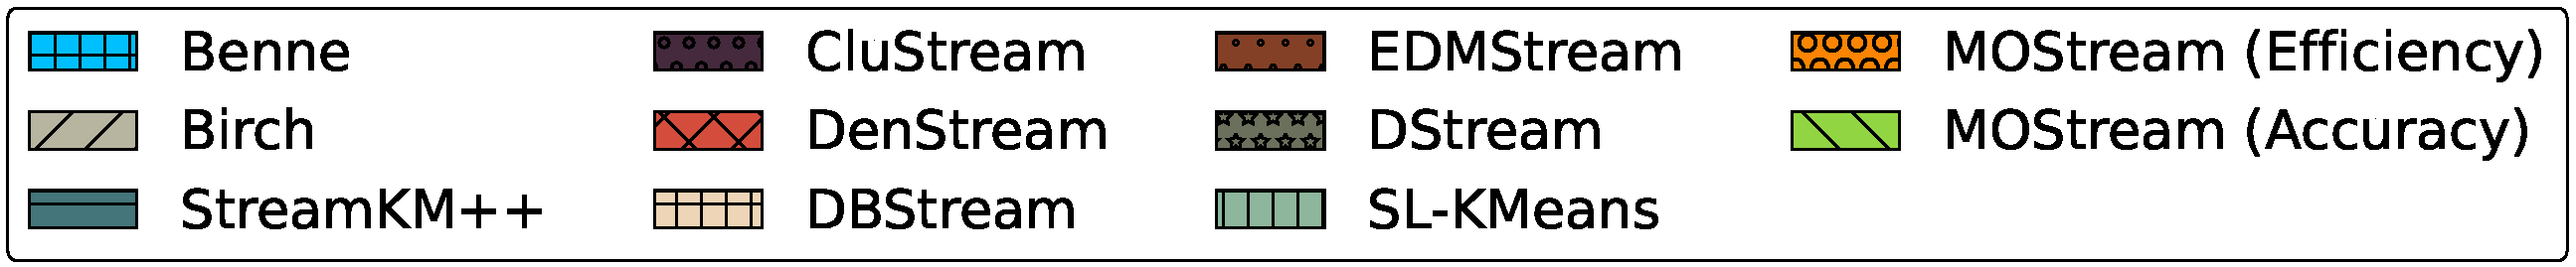
\includegraphics[width=1\linewidth]{Figures/Experiment/General/Purity_Legend.pdf}		
	\end{minipage}
	\begin{subfigure}{.24\textwidth}
        \centering
        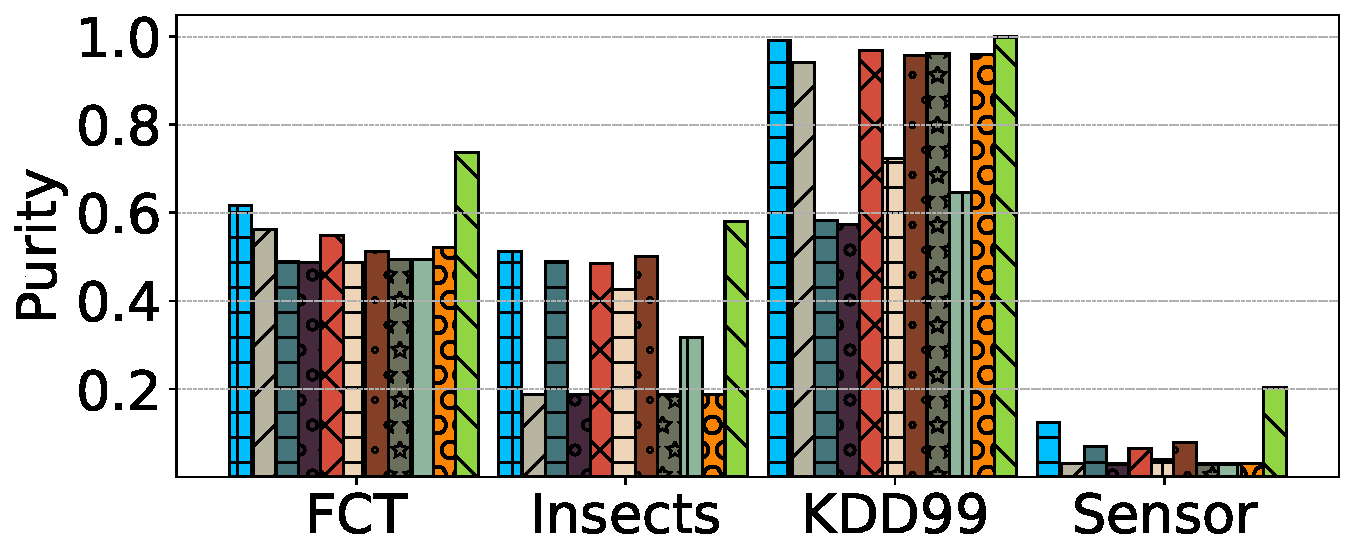
\includegraphics[width=\linewidth]{Figures/Experiment/General/Purity_Real_Existing.pdf}      
         \caption{Accuracy}
         \label{fig:general_purity}
	\end{subfigure}       
  	\begin{subfigure}{.235\textwidth}
        \centering
        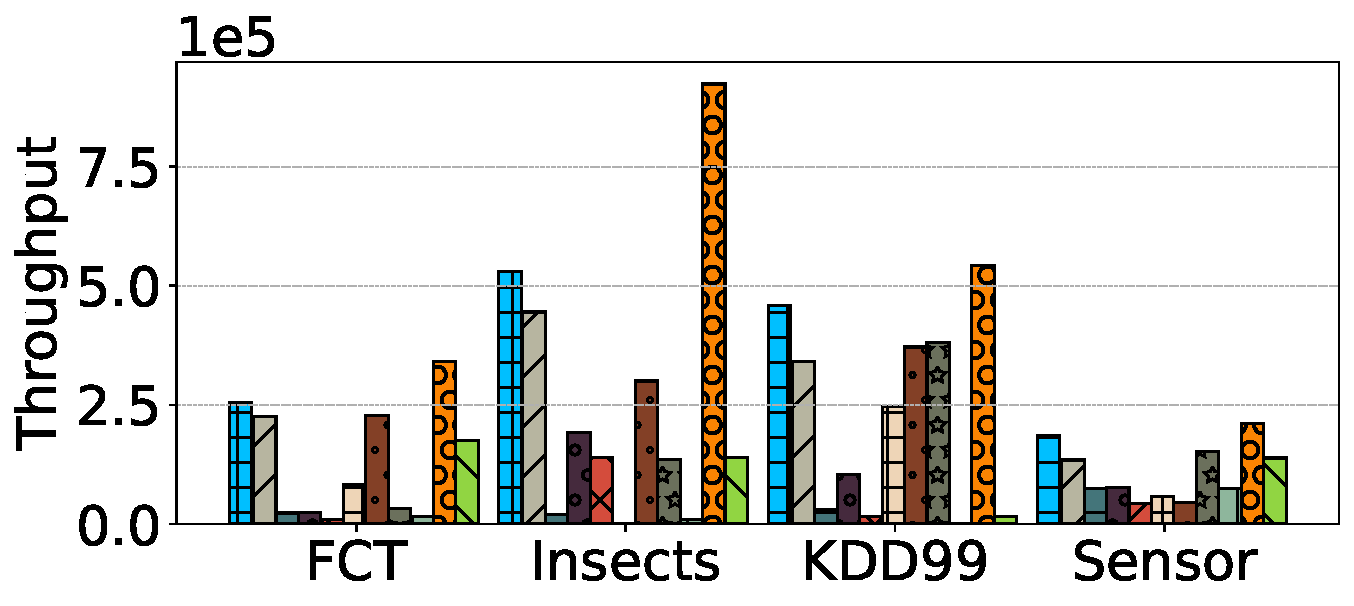
\includegraphics[width=\linewidth]{Figures/Experiment/General/Throughput_Real_Existing.pdf}
        \caption{Efficiency}
        \label{fig:general_throughput}
	\end{subfigure}     
    \caption{Performance Comparison on Four Real-world Workloads. The throughput of \dbstream on \insect dataset and the throughput of \slkmeans on \kdd dataset are much lower than other baselines thus neglected to be shown in the figure.}
    \label{fig:general_comparison}
\end{figure}
 
\subsection{General Evaluation of Clustering Behavior}
\label{subsec:static_evaluation}
The versatility of \algo allows it to be configured into two primary variants: \emph{\algo (Accuracy)} and \emph{\algo (Efficiency)}. These variants cater to different optimization objectives based on distinct algorithmic design decisions. We initiate our evaluation by comparing the clustering behavior of these \algo variants with nine existing \dsc algorithms. The evaluation is conducted on four real-world datasets—\fct, \kdd, \insect, and \sensor. The outcomes are illustrated in Figure~\ref{fig:general_comparison}. We can see that \emph{\algo} (Accuracy) attains state-of-the-art purity across all four real-world datasets. Conversely, \emph{\algo (Efficiency)} exhibits purity levels comparable to existing algorithms but surpasses them in throughput. These observations confirm that by judiciously selecting and integrating different design elements, \algo can either optimize for accuracy or efficiency. However, achieving both optimal accuracy and efficiency simultaneously remains elusive, corroborating our analysis regarding the trade-off between these two metrics.


\subsection{Clustering over Varying Workload Characteristics}
\label{subsec:dynamic_evaluation}
We now use three datasets \eds, \ods, and \dimension to evaluate the impact of varying workload characteristics.
Results are shown in Figure~\ref{fig:evolve_comparison} and Figure~\ref{fig:dim_comparison}.

\underline{First}, By evaluating \eds and \ods workloads, we show that \emph{\algo (Accuracy)} and \emph{\algo (Efficiency)} maintain their respective optimization targets even under frequent cluster or outlier evolution. This stability contrasts with the deteriorating performance observed in several existing \dsc algorithms, such as \clustream and \slkmeans, which struggle to adapt to evolving conditions. We attribute this resilience to \algo's dynamic composition capability. Unlike most existing algorithms, \algo continuously monitors stream characteristics to detect any changes, thereby enabling timely and accurate adaptations to the evolving data stream. This dynamic adaptability ensures superior clustering performance under varying conditions.

\underline{Second}, we next evaluate the impact of varying dimensions, utilizing the \dimension workload for this purpose. This workload comprises datasets with dimensions ranging from 20 to 100, as detailed in Table~\ref{tab:Workload}. Since existing baselines all predefined the dimensionality of the processed streaming data and unable to adjust it during the clustering process, we only conduct the comparison between the two variants of \algo. The outcomes of this evaluation are graphically represented in Figure~\ref{fig:dim_comparison}. Remarkably, \algo maintains a stable purity level of approximately 0.4 across datasets with diverse dimensions. While this purity level may not be high, its consistency is noteworthy, particularly when contending with the \emph{Curse of Dimensionality}. Operations integral to clustering—such as updating the summarizing data structure and pinpointing the appropriate cluster for data insertion—are intrinsically reliant on distance calculations involving the original high-dimensional data. The efficacy of these distance metrics tends to wane as the dimensionality escalates, thereby exacerbating the challenge of distinguishing between data points in high-dimensional spaces. Additionally, we discern a decrement in \algo's efficiency concomitant with an increase in the dataset's dimensionality. Our analysis ascertains that the computational complexity of several pivotal operations—including but not limited to the updating of the summarizing data structure and the selection of suitable clusters for data insertion—is directly influenced by the dimensionality of the workload. Consequently, a surge in dimensionality incurs a proportional rise in the computational time required for these operations, thereby attenuating the overall efficiency of the clustering process.



\begin{figure}[t]
	\begin{minipage}{1\linewidth}
		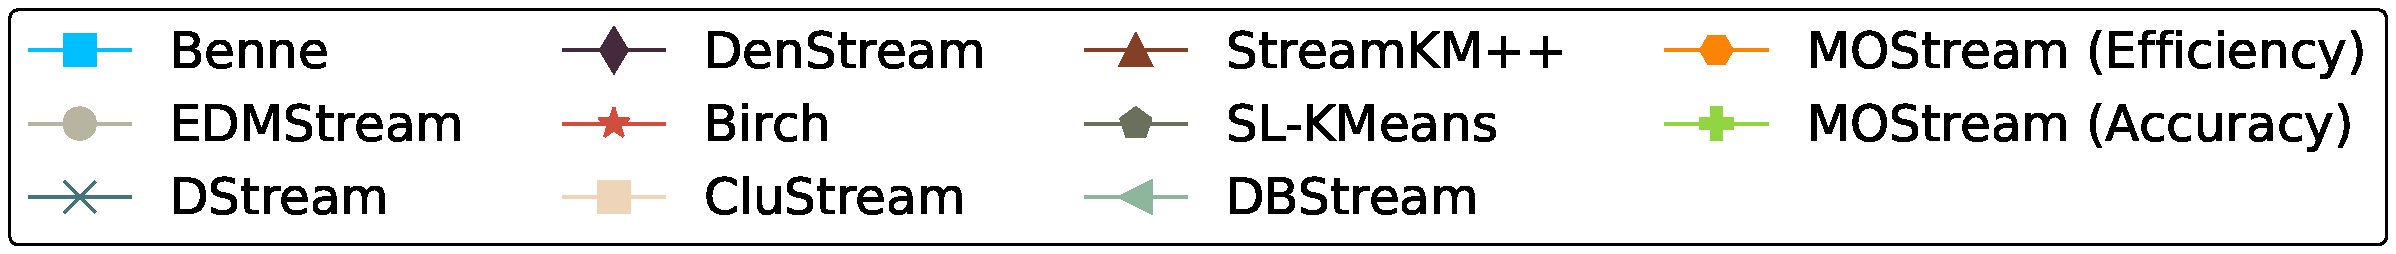
\includegraphics[width=1\linewidth]{Figures/Experiment/EDS/CMM_Legend.pdf}		
	\end{minipage}
 
	\begin{subfigure}{.245\textwidth}
        \centering
        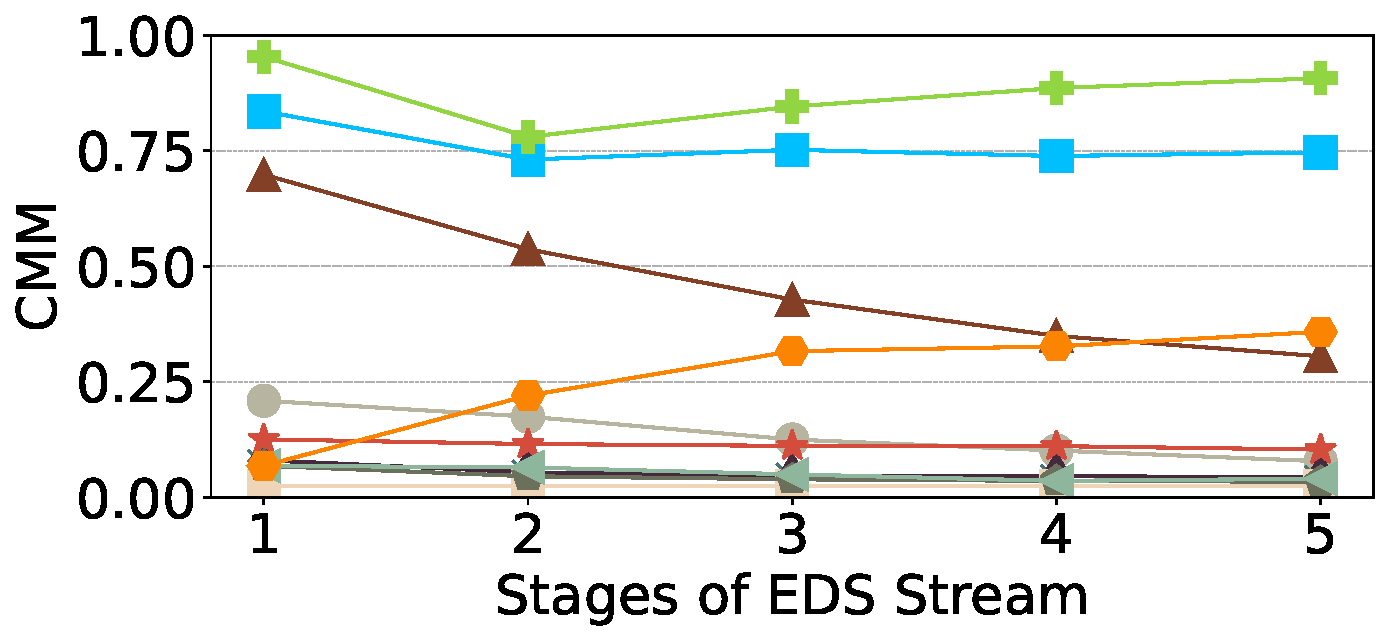
\includegraphics[width=\linewidth]{Figures/Experiment/EDS/EDS_CMM.pdf}      
         \caption{\eds Accuracy}
         \label{fig:eds_cmm}
	\end{subfigure}       
  	\begin{subfigure}{.23\textwidth}
        \centering
        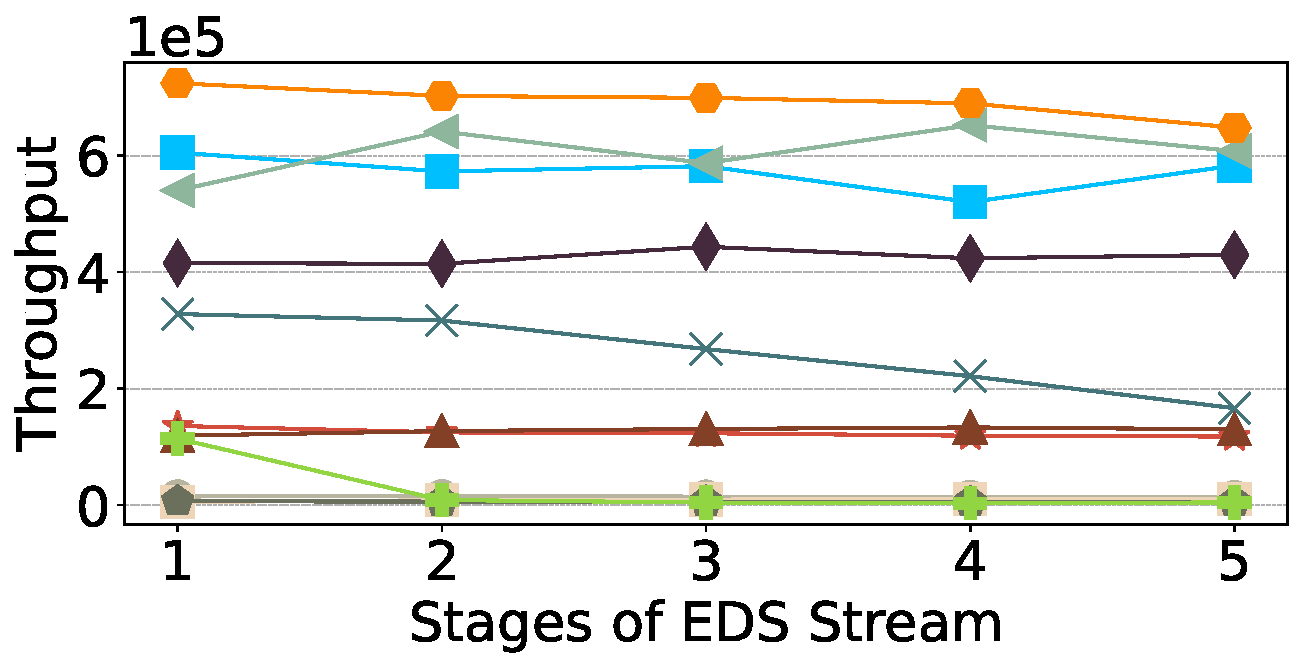
\includegraphics[width=\linewidth]{Figures/Experiment/EDS/EDS_throughput.pdf}
        \caption{\eds Efficiency}
        \label{fig:eds_throughput}
	\end{subfigure}  
 \begin{subfigure}{.245\textwidth}
        \centering
        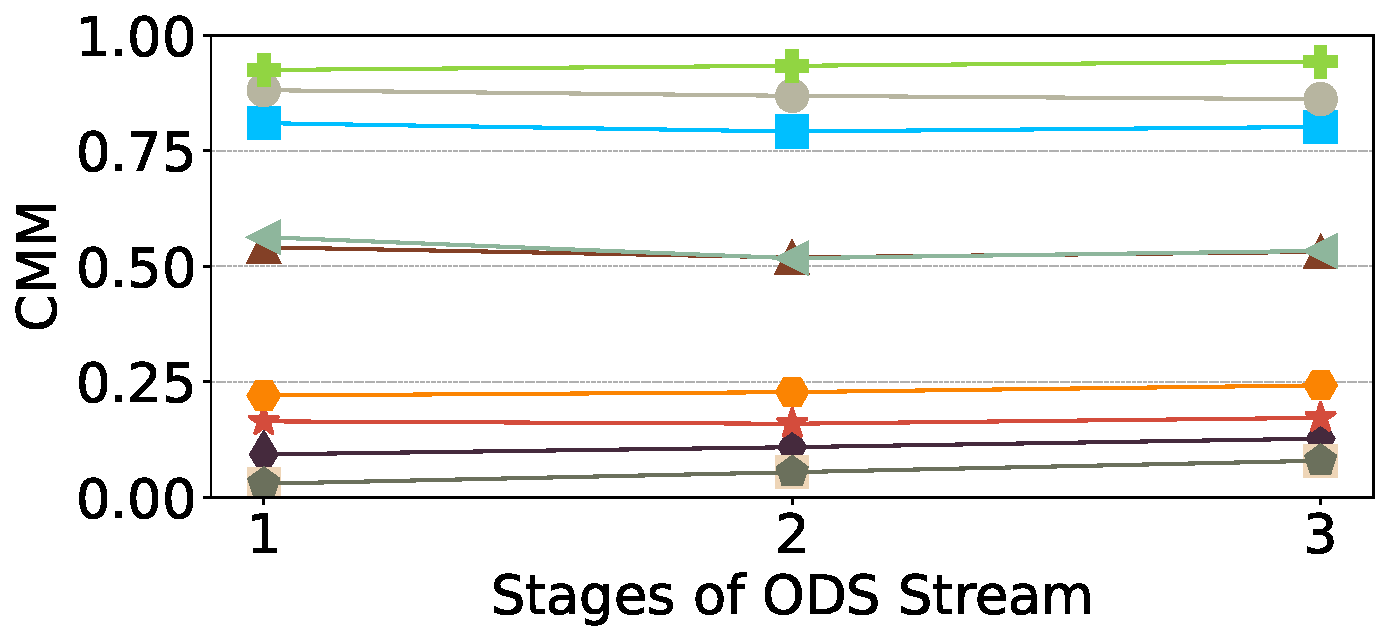
\includegraphics[width=\linewidth]{Figures/Experiment/ODS/ODS_Purity.pdf}      
         \caption{\ods Accuracy}
         \label{fig:ods_purity}
	\end{subfigure}       
  	\begin{subfigure}{.238\textwidth}
        \centering
        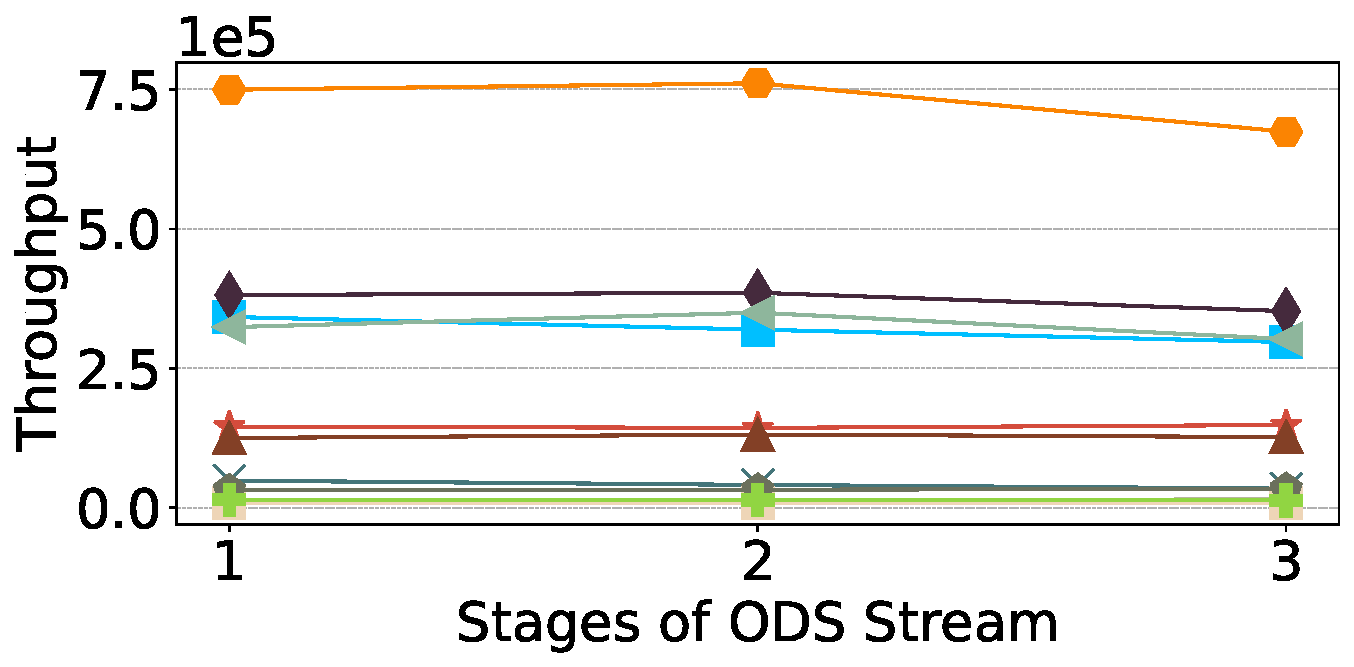
\includegraphics[width=\linewidth]{Figures/Experiment/ODS/ODS_throughput.pdf}
        \caption{\ods Efficiency}
        \label{fig:ods_throughput}
	\end{subfigure}  
    \caption{Performance Comparison on \eds (Figure (a), (b)) and \ods (Figure (c), (d)) workloads with varying cluster or outlier evolution frequency. \eds is divided into five main stages according to the cluster evolution frequency that increases with the increase of the stages.  \ods is divided into three main stages according to the outlier evolution frequency that increases with the increase of the stages.}
        \label{fig:evolve_comparison}
\end{figure}






\begin{figure}[t]
	\centering
	\begin{minipage}{1\linewidth}
        \centering
		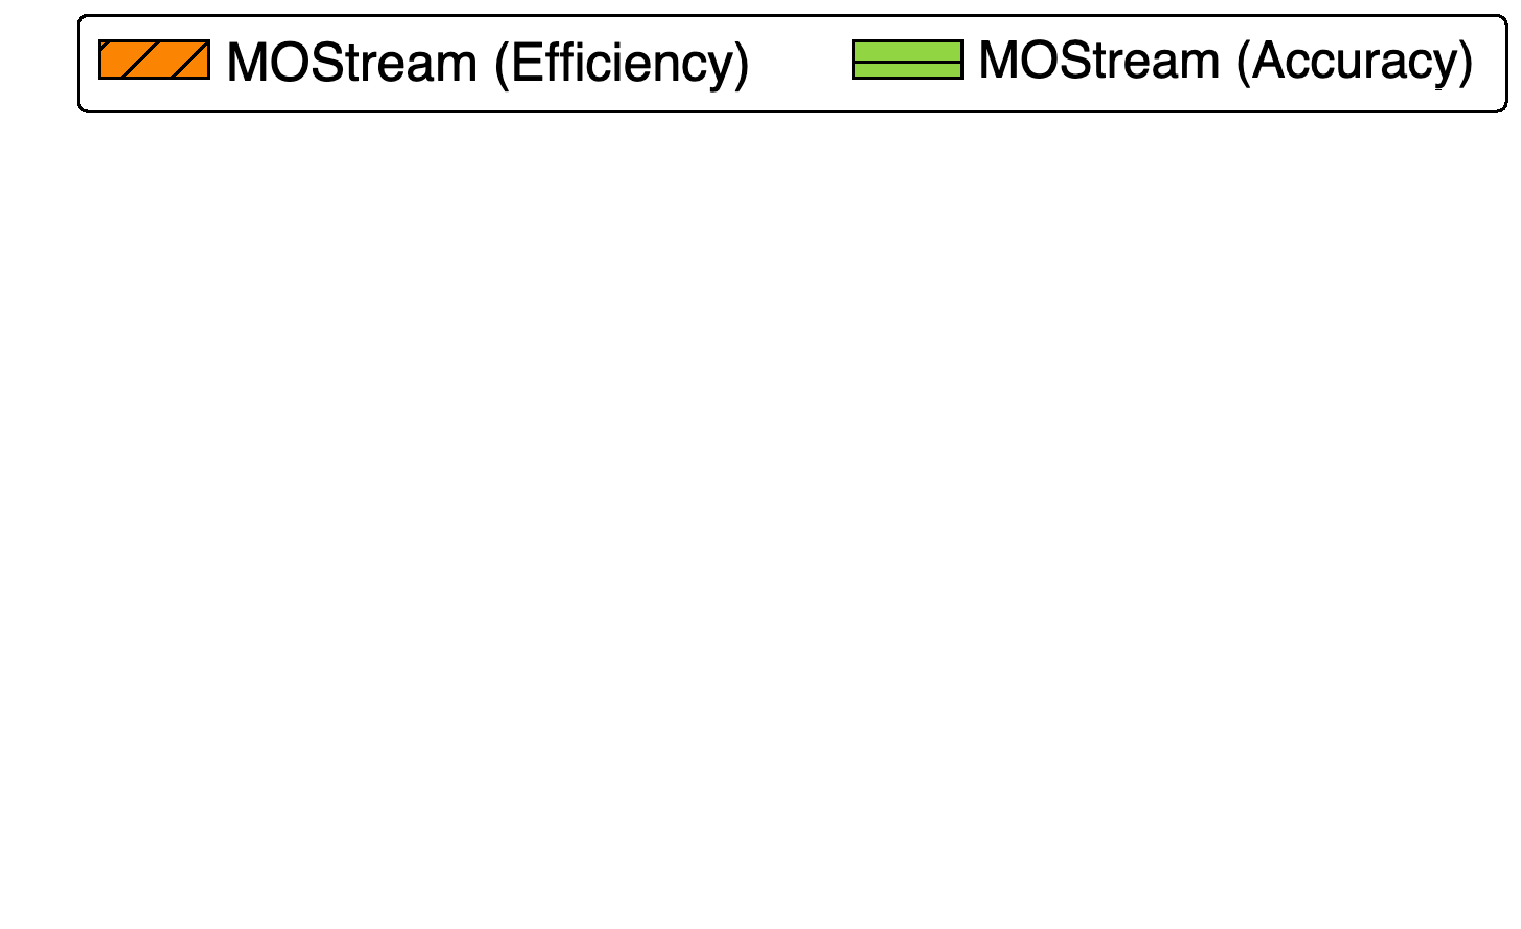
\includegraphics[width=0.7\linewidth]{Figures/Experiment/Dim/Dim_Legend.pdf}		
	\end{minipage}
	\begin{subfigure}{.245\textwidth}
        \centering
        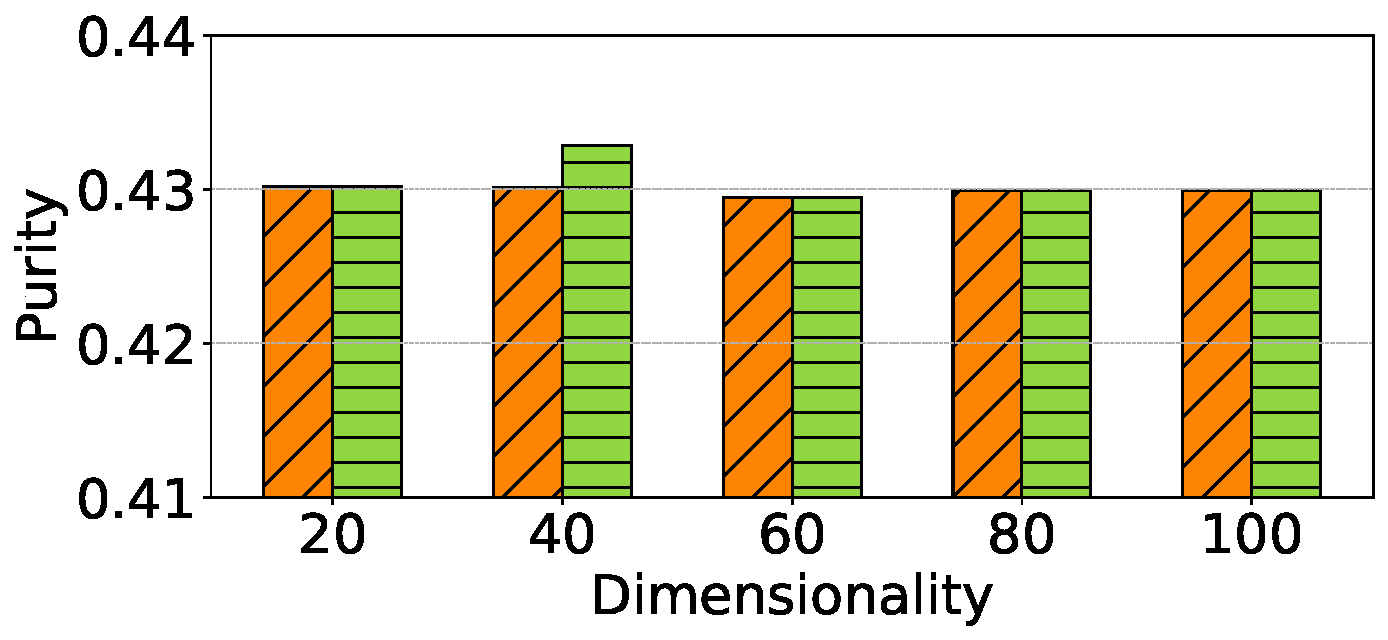
\includegraphics[width=\linewidth]{Figures/Experiment/Dim/Purity_Dim.pdf}      
         \caption{Accuracy}
         \label{fig:dim_purity}
	\end{subfigure}       
  	\begin{subfigure}{.235\textwidth}
        \centering
        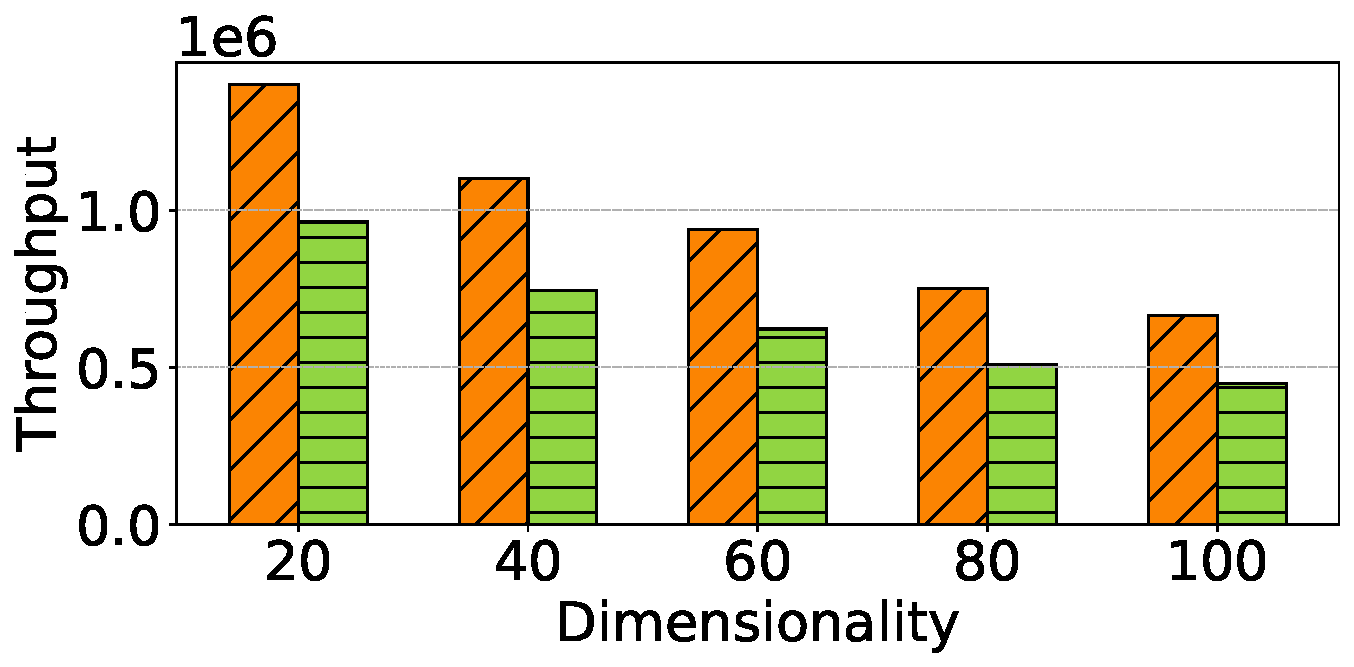
\includegraphics[width=\linewidth]{Figures/Experiment/Dim/Throughput_Dim.pdf}
        \caption{Efficiency}
        \label{fig:dim_throughput}
	\end{subfigure}     
        \caption{Performance Comparison on \dimension workload with varying dimensionality.}
        \label{fig:dim_comparison}	
\end{figure}







% \begin{figure*}[t]
% 	\centering
% 	\begin{minipage}{0.7\linewidth}
% 		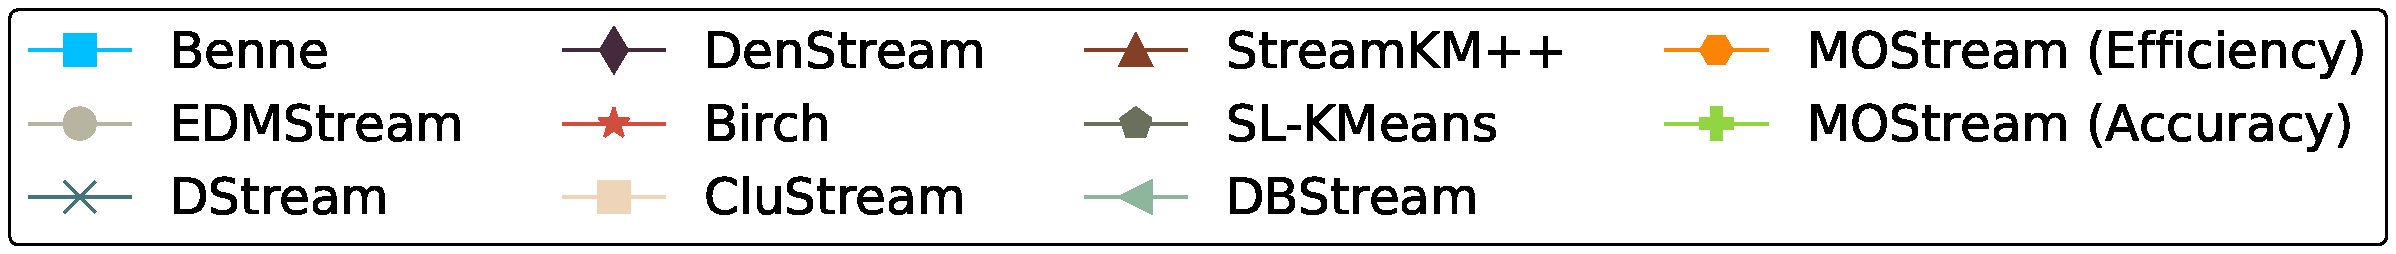
\includegraphics[width=1\linewidth]{Figures/Experiment/EDS/CMM_Legend.pdf}		
% 	\end{minipage}
 
% 	\begin{subfigure}{.25\textwidth}
%         \centering
%         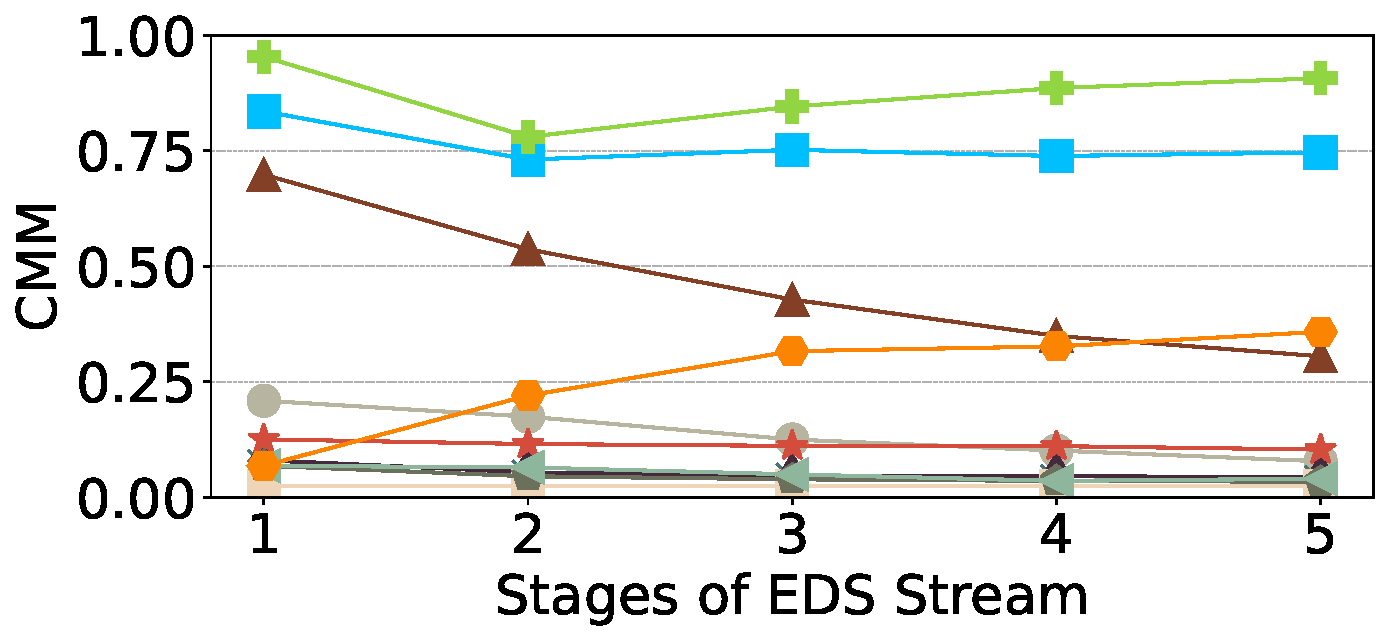
\includegraphics[width=\linewidth]{Figures/Experiment/EDS/EDS_CMM.pdf}      
%          \caption{\eds Accuracy}
%          \label{fig:eds_cmm}
% 	\end{subfigure}       
%   	\begin{subfigure}{.24\textwidth}
%         \centering
%         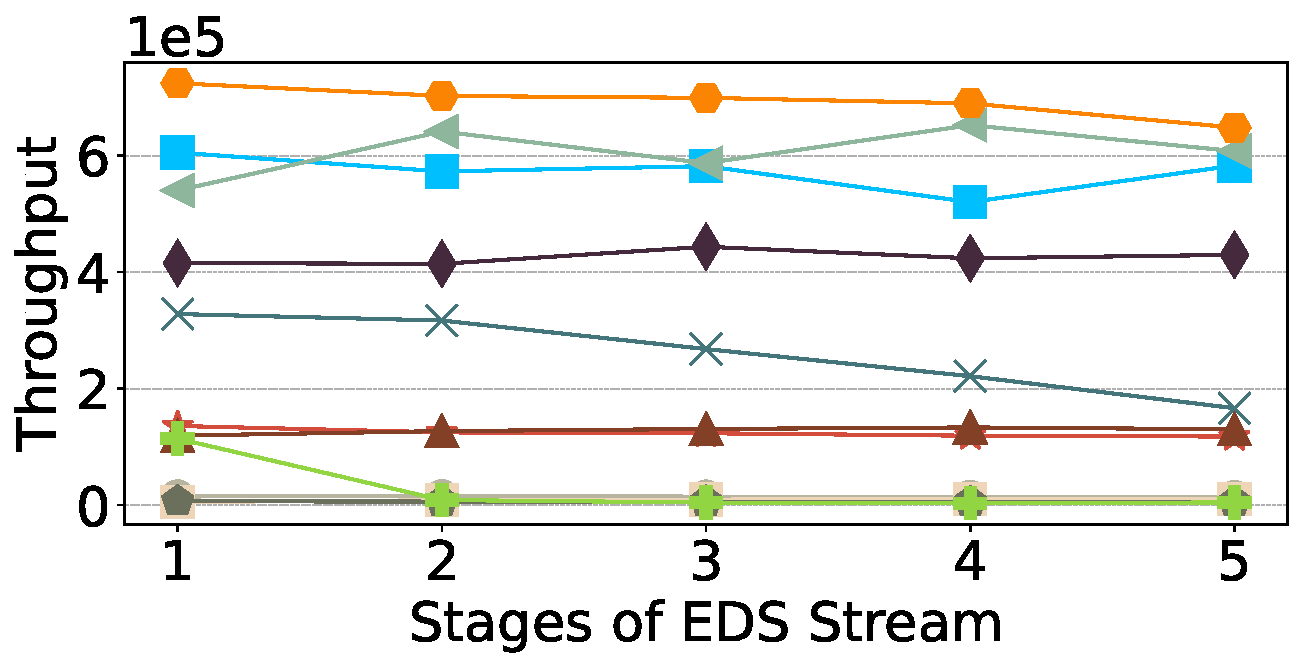
\includegraphics[width=\linewidth]{Figures/Experiment/EDS/EDS_throughput.pdf}
%         \caption{\eds Efficiency}
%         \label{fig:eds_throughput}
% 	\end{subfigure}  
%  \begin{subfigure}{.25\textwidth}
%         \centering
%         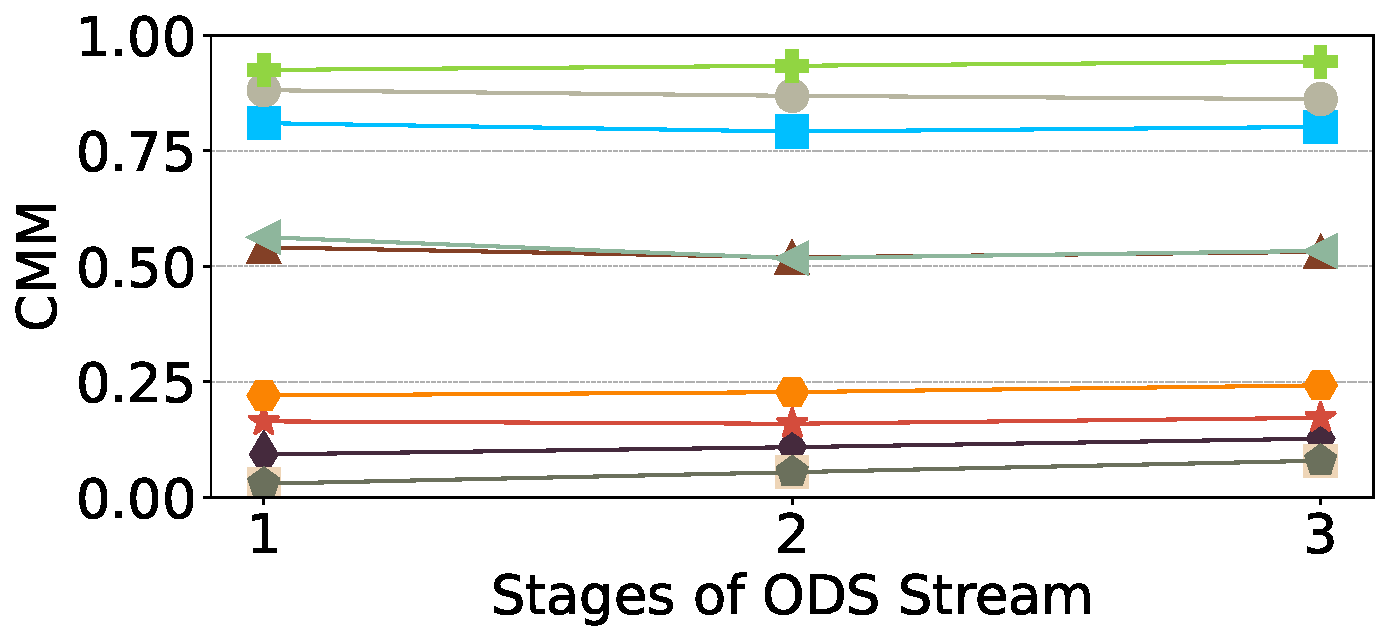
\includegraphics[width=\linewidth]{Figures/Experiment/ODS/ODS_Purity.pdf}      
%          \caption{\ods Accuracy}
%          \label{fig:ods_purity}
% 	\end{subfigure}       
%   	\begin{subfigure}{.24\textwidth}
%         \centering
%         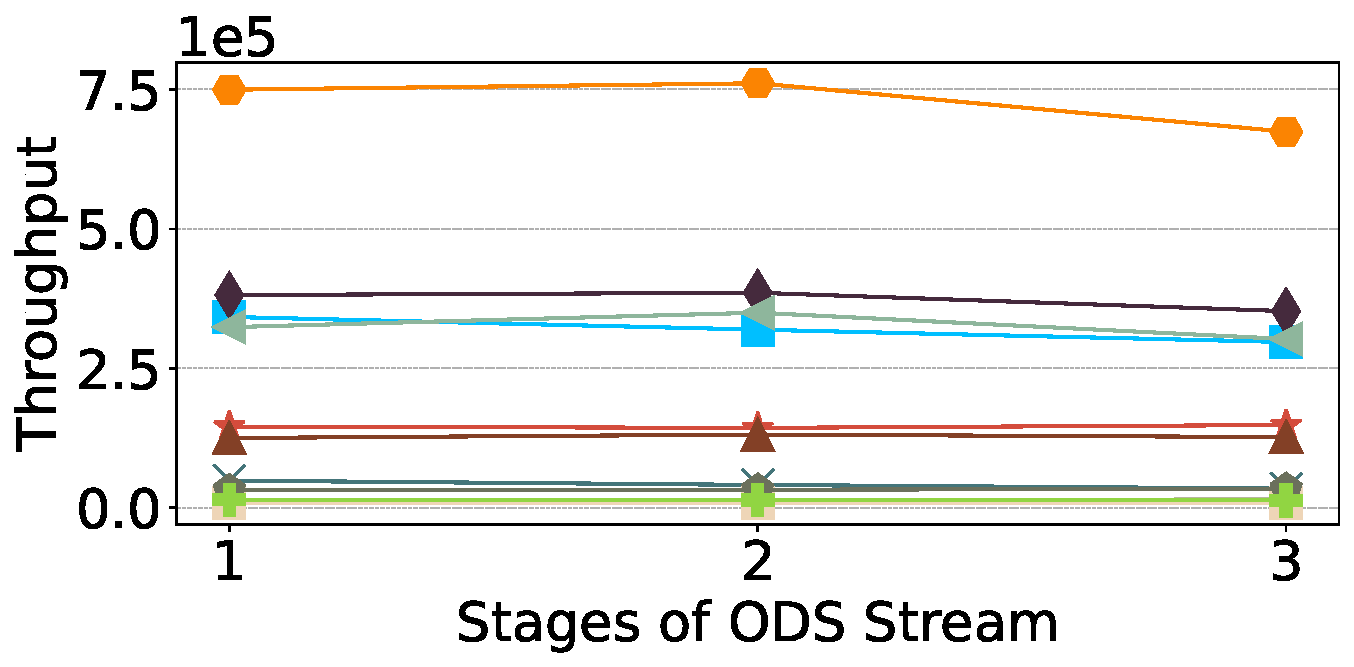
\includegraphics[width=\linewidth]{Figures/Experiment/ODS/ODS_throughput.pdf}
%         \caption{\ods Efficiency}
%         \label{fig:ods_throughput}
% 	\end{subfigure}   
%         \caption{Performance Comparison on \eds (Figure (a), (b)) and \ods (Figure (c), (d)) workloads with varying cluster or outlier evolution frequency. \eds is divided into five main stages according to the cluster evolution frequency that increases with the increase of the stages.  \ods is divided into three main stages according to the outlier evolution frequency that increases with the increase of the stages.}
%         \label{fig:evolve_comparison}
% \end{figure*}
 
\subsection{Empirical Evaluation of Dynamic Composition Ability}
We conducted an empirical evaluation to demonstrate the effectiveness of \algo's dynamic composition abilities, including regular stream characteristics detection (Section~\ref{subsec:regular-detection}), automatic choice selection (Section~\ref{subsec:auto-selection}) and flexible algorithm migration (Section~\ref{subsec:migration}) respectively under evolving workload characteristics. 
To assess the role of the regular stream characteristics detection module, we estimated the general location where the stream characteristics evolve in the workload and checked whether the evolution was detected timely and accurately based on the output of \algo's regular detection function, as discussed in Algorithm~\ref{algo:auto_detection}. To evaluate the effectiveness of the automatic choice selection and flexible algorithm migration modules, we introduced two additional variants: \algo \textit{(Accuracy) without migration} and \algo \textit{(Efficiency) without selection}. By comparing the changes in both purity and throughput across these four variants of \algo, we identified the specific contributions of the automatic choice selection and flexible migration modules to the overall dynamic composition capability.

\begin{figure}[t]
	\centering
 \begin{minipage}{0.8\linewidth}
		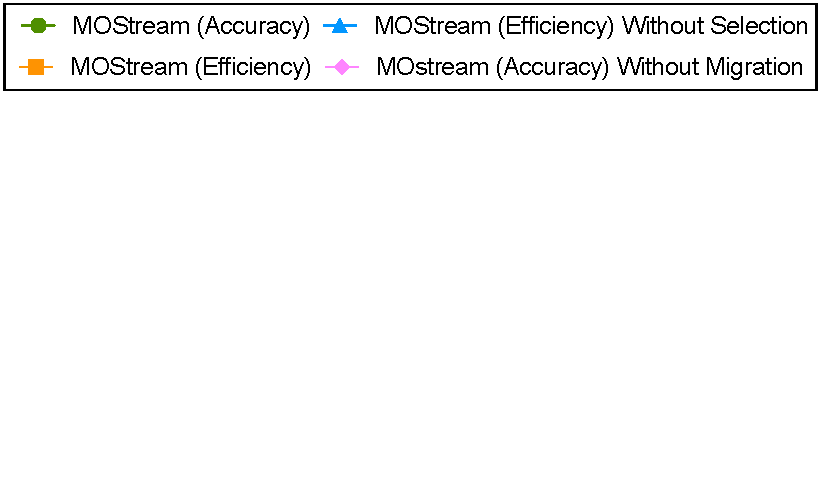
\includegraphics[width=1\linewidth]{Figures/Experiment/Dynamic/Legend.pdf}		
	\end{minipage}
 
	\begin{subfigure}{.235\textwidth}
        \centering
        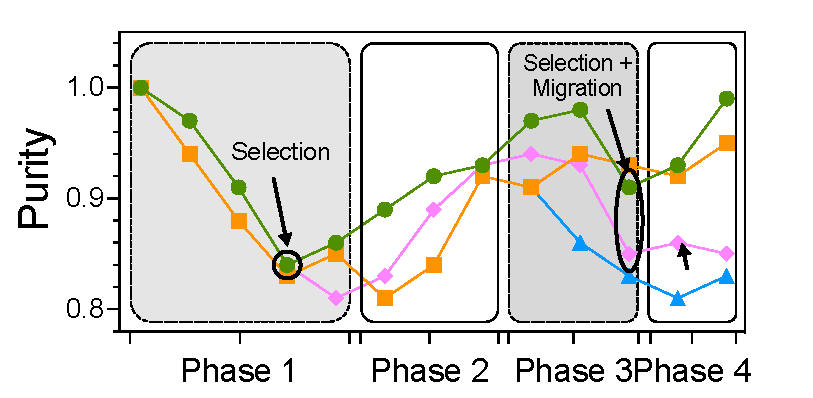
\includegraphics[width=\linewidth]{Figures/Experiment/Dynamic/PurityonKDD99.pdf}      
         \caption{Accuracy}
         \label{fig:dynamic_purity_kdd}
	\end{subfigure}       
  	\begin{subfigure}{.245\textwidth}
        \centering
        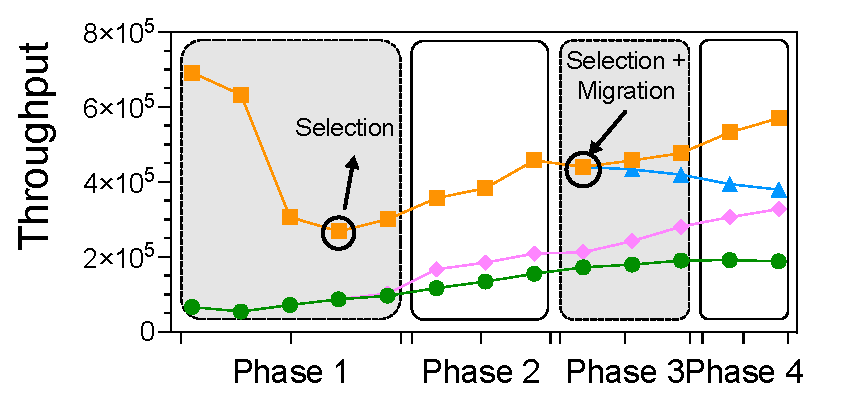
\includegraphics[width=\linewidth]{Figures/Experiment/Dynamic/ThroughputonKDD99.pdf}
        \caption{Efficiency}
        \label{fig:dynamic_throughput_kdd}
	\end{subfigure}     
    \caption{Detailed performance analysis of \algo's variants on \kdd. Measurements are taken at intervals of 350,000 data points with 4 phases in total.}
    \label{fig:dynamic_real_comparison}
\end{figure}

\subsubsection{Composition Effectiveness Study}
We commence by evaluating the performance of the four \algo variants on the real-world \kdd workload, characterized by a high frequency of outlier evolution and low but increasing frequency of cluster evolution. Measurements are taken at intervals of 350,000 data points with 4 phases in total, capturing both clustering outcomes and workload characteristic evolutions, as illustrated in Figure~\ref{fig:dynamic_real_comparison}. Notably, \algo (Accuracy) excels in purity, while \algo (Efficiency) demonstrates superior throughput, each aligning with their respective optimization objectives. Three key observations emerge from this analysis.

\underline{First}, a synchronized examination of \algo's clustering behavior and workload evolution (indicated by grey lines in the figure) reveals that while workload changes adversely affect clustering performance (evident in Phases 1 and 3), both \algo (Accuracy) and \algo (Efficiency) swiftly recover in Phases 2 and 4. For \algo (Accuracy), the initial use of the \damped window model leads to a rapid decline in both purity and throughput during Phase 1 due to its inability to effectively manage increasing outlier frequencies. However, the algorithm's regular stream characteristics detection module, as outlined in Algorithm~\ref{algo:auto_detection}, identifies this issue at the close of Phase 1, prompting a transition to the \landmark window model to better cope with outlier evolution. The subsequent improvement in purity during Phase 2 attests to the efficacy of this module. A similar recovery is observed in Phase 4, where the algorithm switches from \CFT to \MCs to adapt to increasing cluster evolution in Phase 3. For \algo (Efficiency), the algorithm opts to forgo outlier detection to minimize overhead, in line with its optimization target. Consequently, its performance deteriorates in Phases 1 and 2. However, upon entering Phase 3, characterized by high cluster evolution, the algorithm promptly detects this change and switches from \Grids to \DPT, resulting in improved purity and throughput in Phase 4, as depicted in Figure~\ref{fig:dynamic_real_comparison}.

\underline{Second}, apparently, both the purity and throughput drops significantly when canceling the usage of automatic design choice selection and switching, as shown by \algo \textit{(Efficiency) without selection}.  This indicates the limitation of the individual composition
On the contrary, applying the automatic design choice selection into the algorithm can make full use of the strengths of every design choices, leading to both better clustering accuracy and efficiency, as shown by \algo (Efficiency). \underline{Third}, the inclusion of migration in the algorithm improves accuracy at the expense of clustering speed. A comparative analysis of \algo (Accuracy) and \algo \textit{(Accuracy) without migration} reveals that while the former consistently outperforms the latter in purity, it lags in throughput. A detailed assessment of the overhead incurred by the three dynamic composition modules will be presented in the subsequent section.

\subsubsection{Analysis of Composition-Related Overhead}
We proceed to examine the computational overhead associated with \algo's two pivotal composition procedures: detection and migration. This is juxtaposed against the time expended on clustering, contingent on the selected composition. As illustrated in Figure~\ref{fig:etb_analysis}, the time allocation for both detection and migration is relatively minimal for \algo (Accuracy) in comparison to the primary clustering task. This underscores the efficiency of these composition procedures.
In the case of \algo (Efficiency), the scenario is somewhat different. Given that this variant is optimized for speed, the clustering operation itself is more time-efficient. Consequently, the proportion of time spent on the detection procedure appears to be larger relative to \algo (Accuracy). However, it's crucial to note that \algo (Efficiency) omits the migration procedure altogether, as elaborated in Section~\ref{subsec:migration}. This strategic omission further enhances its efficiency, aligning it closely with its optimization objectives.
This analysis confirms that the overheads associated with dynamic composition in \algo are well-contained, thereby not compromising the algorithm's primary objectives of either accuracy or efficiency.

\begin{figure}[t]
	\centering
	\begin{minipage}{1\linewidth}
        \centering
		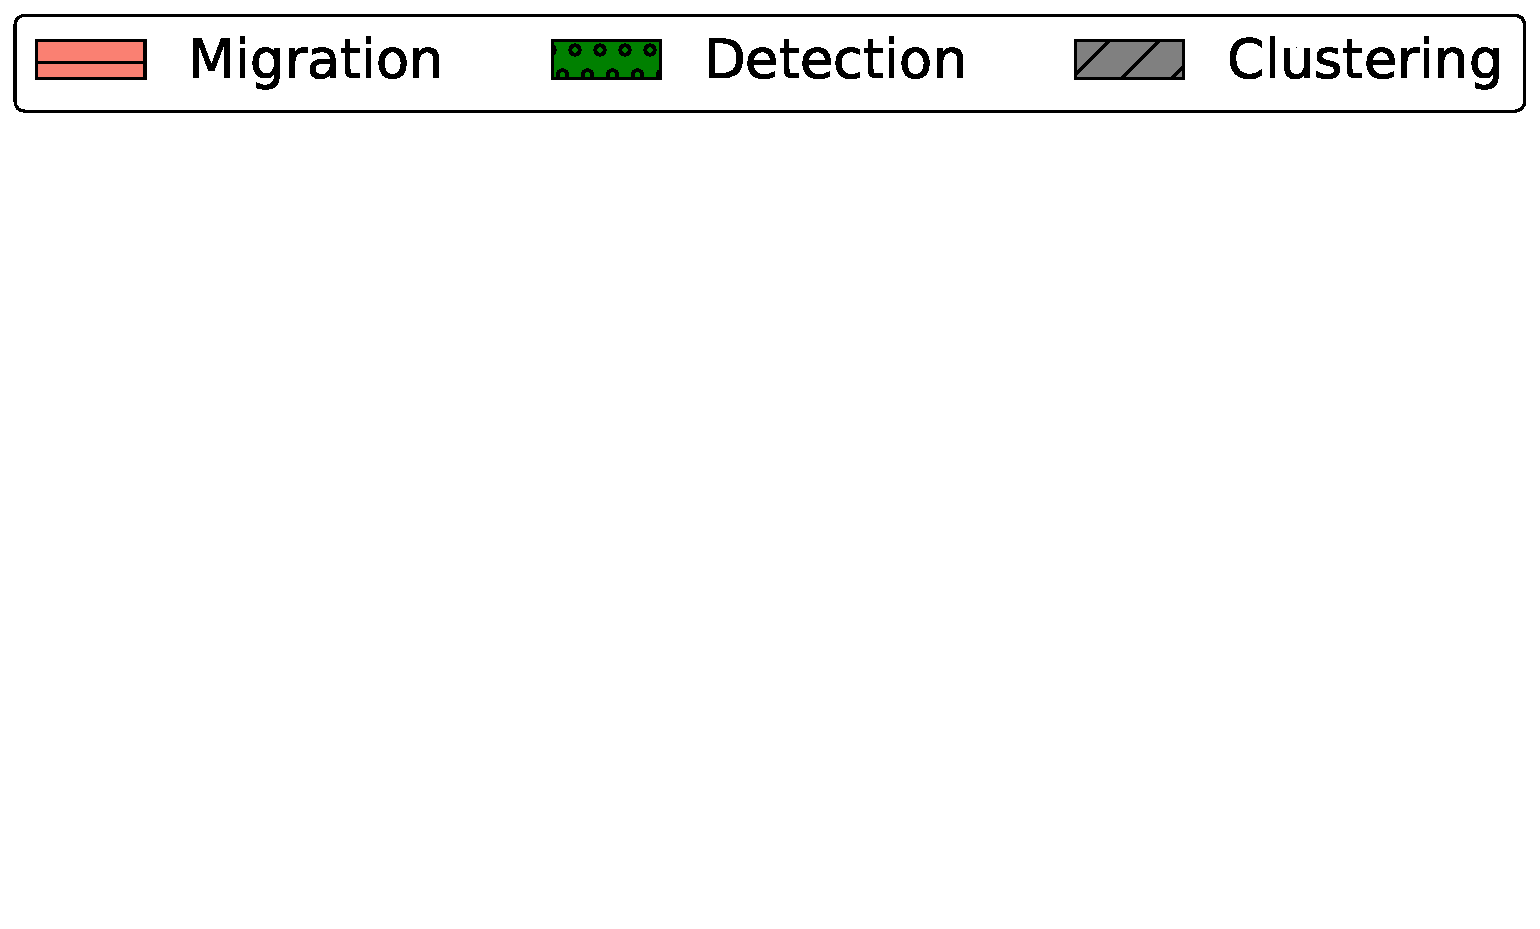
\includegraphics[width=0.7\linewidth]{Figures/Experiment/ETB/Execution_Time_Legend.pdf}		
	\end{minipage}
	\begin{subfigure}{.24\textwidth}
        \centering
        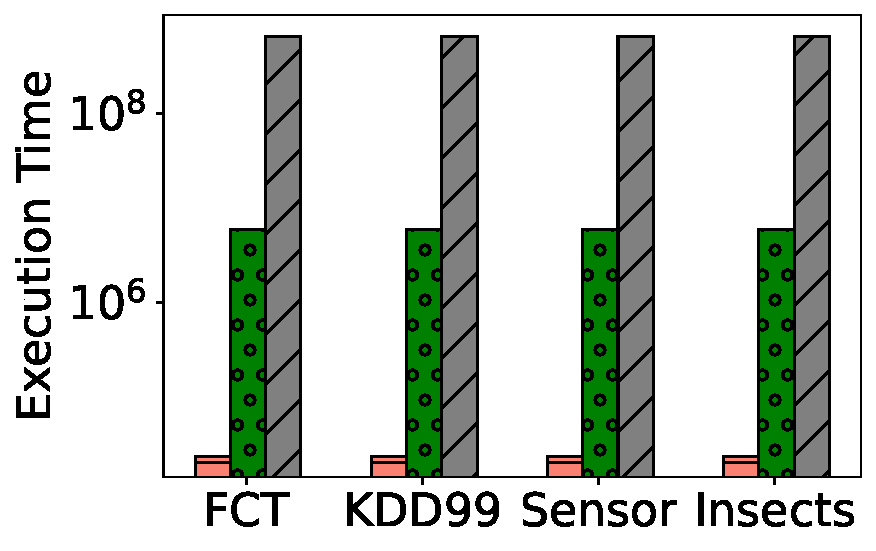
\includegraphics[width=\linewidth]{Figures/Experiment/ETB/Execution_Time_Acc.pdf}      
         \caption{\algo (Accuracy)}
         \label{fig:etb_purity}
	\end{subfigure}       
  	\begin{subfigure}{.24\textwidth}
        \centering
        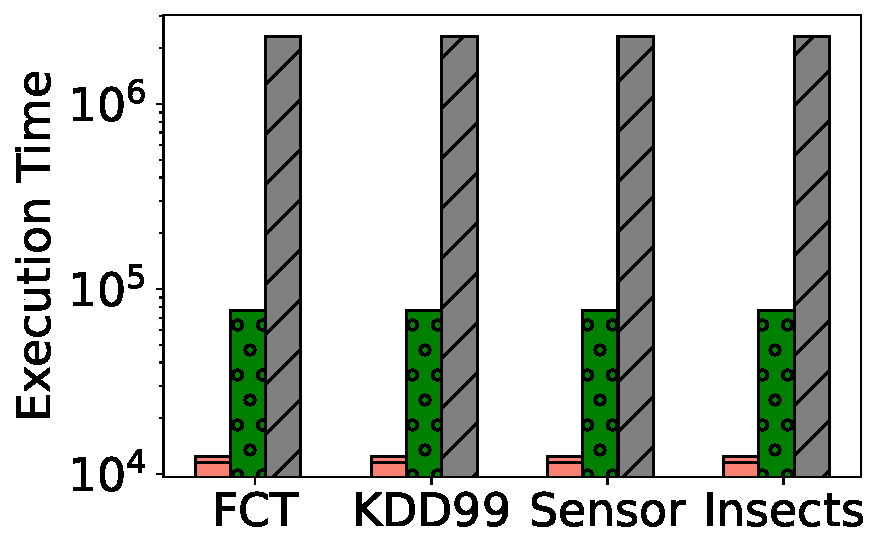
\includegraphics[width=\linewidth]{Figures/Experiment/ETB/Execution_Time_Eff.pdf}
        \caption{\algo (Efficiency)}
        \label{fig:etb_throughput}
	\end{subfigure}     
        \caption{Execution Time Break Down Analysis on Real-world Workloads of two \algo variants.}
        \label{fig:etb_analysis}	
\end{figure}

% \subsection{Scalability Across Dimensions}
% We turn our attention to evaluating the scalability of \algo in the context of varying dimensions, utilizing the \dimension workload for this purpose. This workload comprises datasets with dimensions ranging from 20 to 100, as detailed in Table~\ref{tab:Workload}. The outcomes of this evaluation are graphically represented in Figure~\ref{fig:dim_comparison}.
% %
% Remarkably, \algo maintains a stable purity level of approximately 0.4 across datasets with diverse dimensions. While this purity level may not be high, its consistency is noteworthy, particularly when contending with the \emph{Curse of Dimensionality}. Operations integral to clustering—such as updating the summarizing data structure and pinpointing the appropriate cluster for data insertion—are intrinsically reliant on distance calculations involving the original high-dimensional data. The efficacy of these distance metrics tends to wane as the dimensionality escalates, thereby exacerbating the challenge of distinguishing between data points in high-dimensional spaces.
% %
% Additionally, we discern a decrement in \algo's efficiency concomitant with an increase in the dataset's dimensionality. Our analysis ascertains that the computational complexity of several pivotal operations—including but not limited to the updating of the summarizing data structure and the selection of suitable clusters for data insertion—is directly influenced by the dimensionality of the workload. Consequently, a surge in dimensionality incurs a proportional rise in the computational time required for these operations, thereby attenuating the overall efficiency of the clustering process.

% We now verify dimensionality scalability of \algo on \dimension workload, which contains data with varying dimensions from 20 to 100 as shown in table~\ref{tab:Workload}. The comparison result is shown in figure~\ref{fig:dim_comparison}. 
% \algo achieves consistent purity for handling workloads with varying of dimensions. This is due to the well-known \emph{Curse of Dimensionality} issue. Many of the clustering operations, such as updating the summarizing data structure and searching for the suitable cluster for data insertion are all based on calculating the distance of the original high dimensional data, but distance metric will become less effective to differentiate data points in high dimensional space.
% The efficiency of \algo drops when increasing dimensions in the workload. We observe that the complexity of many operations is highly related to workload dimension, such as updating the summarizing data structure and searching for the suitable cluster for data insertion based on distance. Therefore, with the increase of workload dimension, more time is spent on these operations bringing down the clustering efficiency. 



% Surprisingly, we find that the purity of all of the \dsc algorithms, including the existing ones and the three variants of \algo are very close with each other in handling high dimensional datasets. This leads to a quite different observation from the previous experiments. We attribute this to the well-known \emph{Curse of Dimensionality} issue that higher dimensional workloads are expected to be harder to cluster correctly since the distance metric will become meaningless in high dimensional space. Many of the clustering operations, such as updating the summarizing data structure and searching for the suitable cluster for data insertion are all based on calculating the distance of the original high dimensional data. That is why all of the tested algorithms achieve similar clustering quality on \dimension workload.

% Despite the significant differences among \dsc algorithms, they all achieve lower throughput for higher workload dimensionalities. We observe that the complexity of many operations is highly related to workload dimension, such as updating the summarizing data structure and searching for the suitable cluster for data insertion based on distance. Therefore, with the increase of workload dimension, more time is spent on these operations bringing down the clustering efficiency.  Higher dimensional workloads are expected to be harder to cluster correctly due to the well-known \emph{Curse of Dimensionality} issue. However, we observe that algorithms achieve higher purity for handling high dimensional workloads (\fct and \kdd). We suspect that dimensionality is not a dominant factor for the clustering accuracy here. Nevertheless, we plan to evaluate the impact of dimensionality with more extensive datasets in future.

% [Add some figures]

\subsection{Sensitivity Analysis of Parameters}
We conducted a sensitivity analysis of \algo (Accuracy) and \algo (Efficiency) on \fct workload. As previously delineated, \algo (Accuracy) aims for elevated purity levels, while \algo (Efficiency) targets higher throughput. Both variants fulfill their respective optimization criteria. The results are shown in Figure~\ref{fig:parameter_analysis}.

1) \textbf{Outlier Distance Threshold ($\delta$)}: For each data point $x_t$ and its nearest cluster $C_t$, we compute the distance $D(x_t, C_t)$. If this distance surpasses the threshold $\delta$, $x_t$ is deemed an outlier. We experimented with $\delta$ values from 50 to 950 for \algo (Accuracy) and from 10 to 100 for \algo (Efficiency). Both variants maintain stable purity and throughput levels across this range. Notably, \algo (Accuracy) undergoes a window model transition from 'landmark' to 'damped' when the outlier distance threshold increases within a specific range, causing a sudden alteration in performance metrics, and leads to an increase in cluster size and purity. However, the throughput does not change, and this is due to the fact that both \landmark and \damped are time consuming for clustering. Conversely, \algo (Efficiency) remains unaffected as it does not consider the number of outliers as a performance metric.

2) \textbf{Queue Size Threshold}: We varied the queue size from 20,000 to 100,000. Both variants exhibit a decline in purity as the queue size increases, attributed to less frequent algorithmic adjustments. While the throughput for \algo (Accuracy) diminishes with an increasing queue size due to the growing complexity of its summarizing data structure, \algo (Efficiency) experiences a throughput increase. This is attributed to fewer algorithmic migrations and a transition to a more efficient data structure (\Grids) as the queue size enlarges.

3) \textbf{Variance Threshold}: \algo activates the \textit{characteristics.frequent evolution} flag when the calculated variance of sampled data exceeds a predefined threshold. We tested variance thresholds from 400 to 4,000. As the threshold rises, both purity and throughput for \algo (Accuracy) decline. This is due to the algorithm's assumption of infrequent evaluations at higher variance thresholds, leading to less frequent algorithmic migrations and increased computational overhead. \algo (Efficiency) remains relatively stable across varying variance thresholds. At a high variance threshold of 4,000, both variants achieve similar purity levels, but \algo (Efficiency) outperforms \algo (Accuracy) in throughput due to the absence of algorithmic migrations.

\begin{figure}[t]
	\centering
	\begin{subfigure}{.233\textwidth}
        \centering
        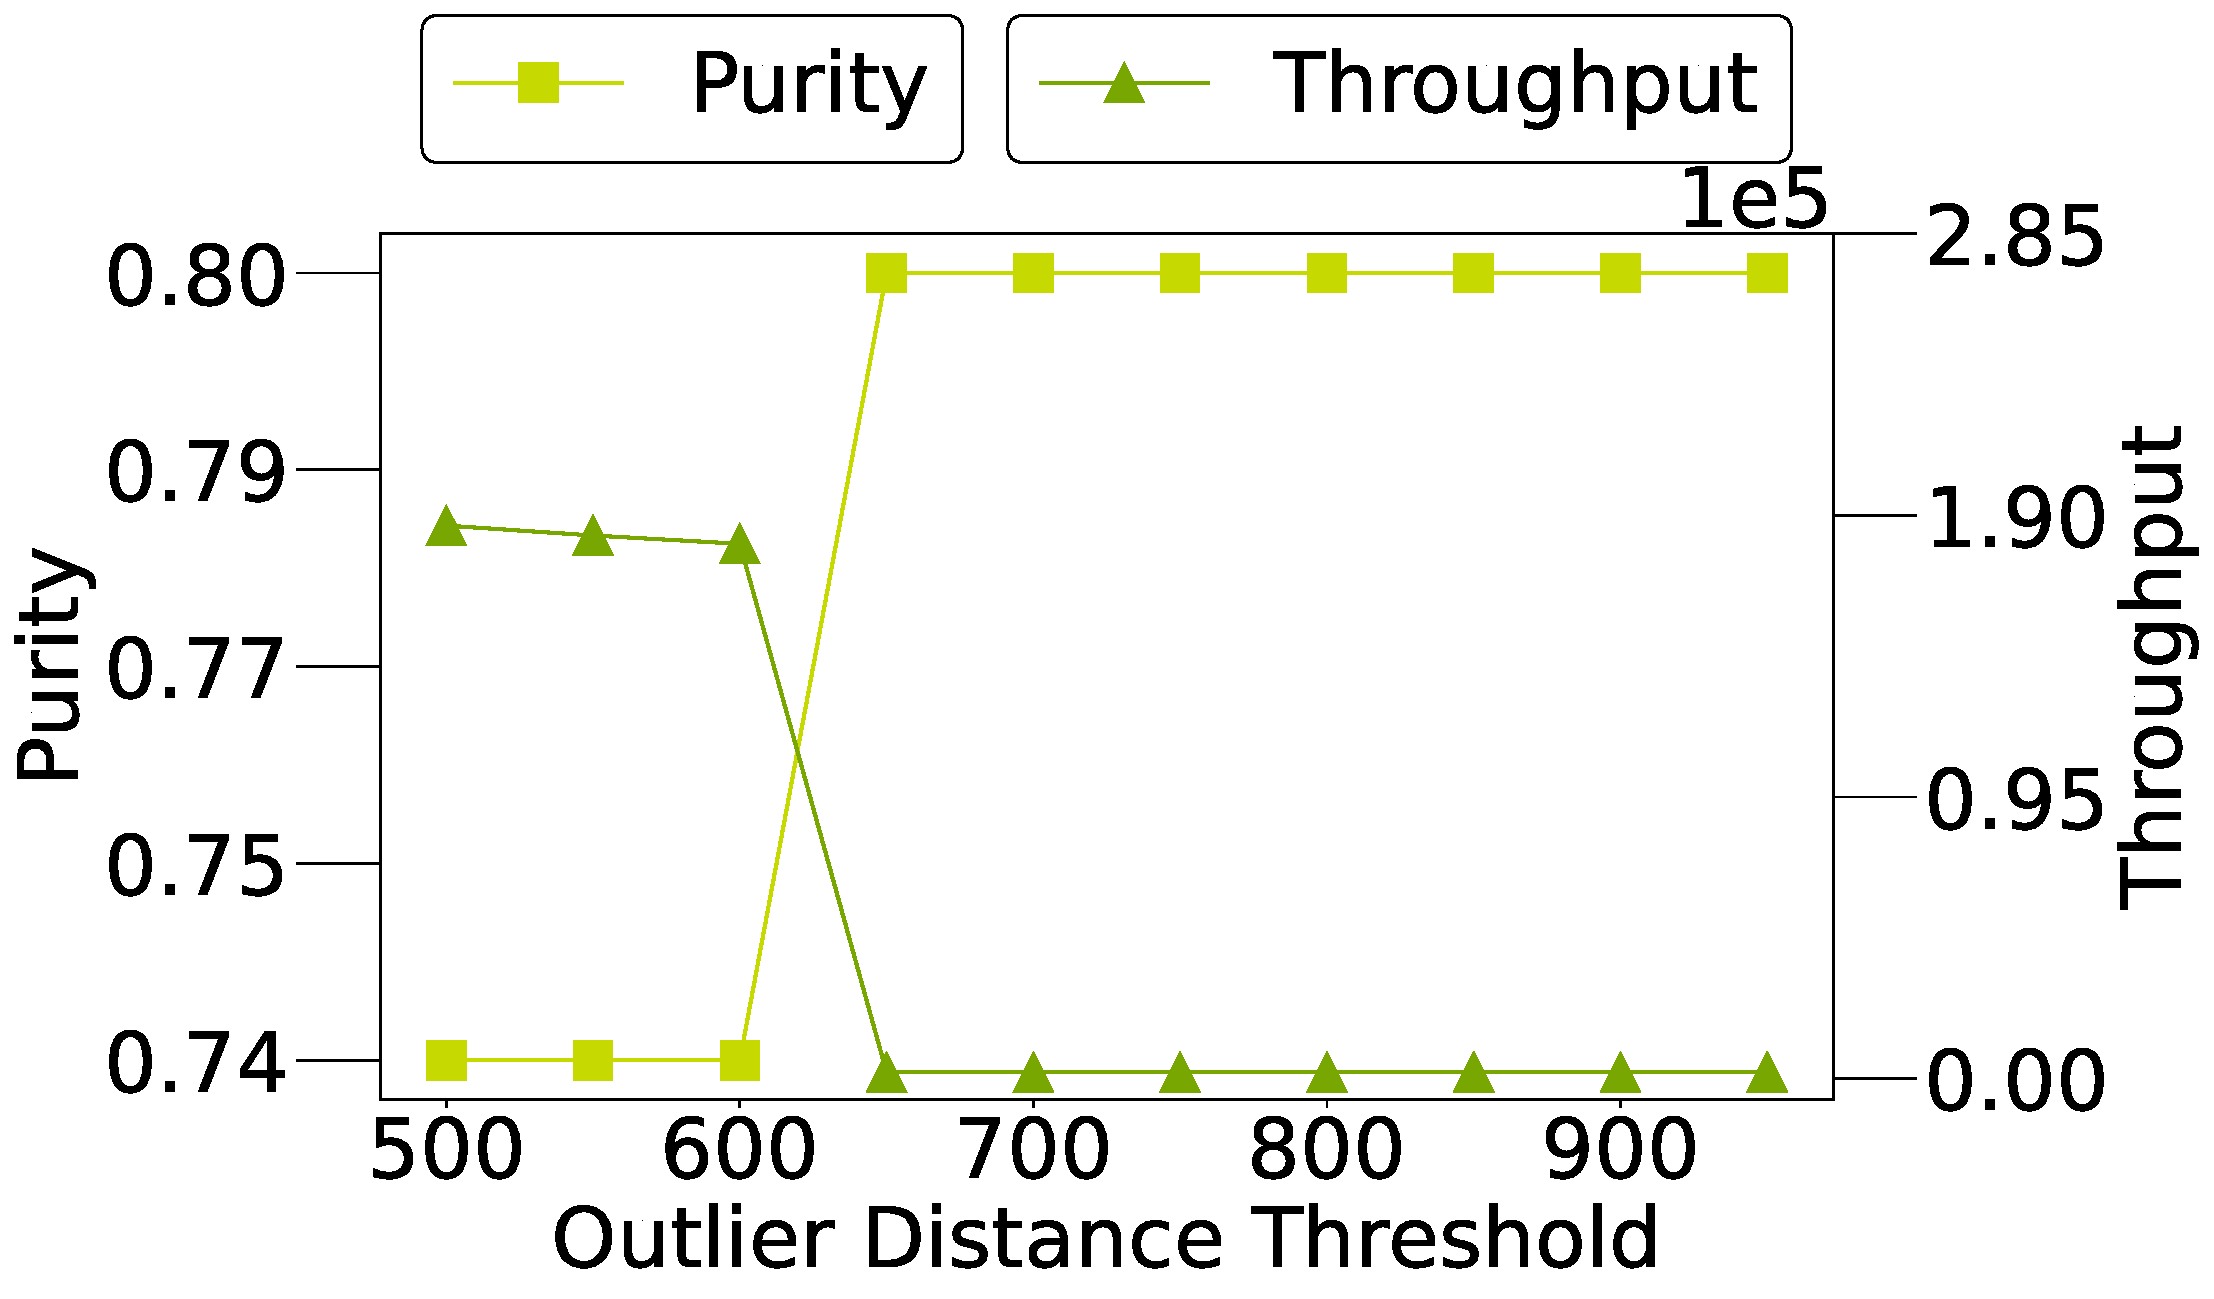
\includegraphics[width=\linewidth]{Figures/Experiment/Param/Config_Outlier_Distance_Acc.pdf}
         \label{fig:outlier_distance_purity}
	\end{subfigure}       
  	\begin{subfigure}{.244\textwidth}
        \centering
        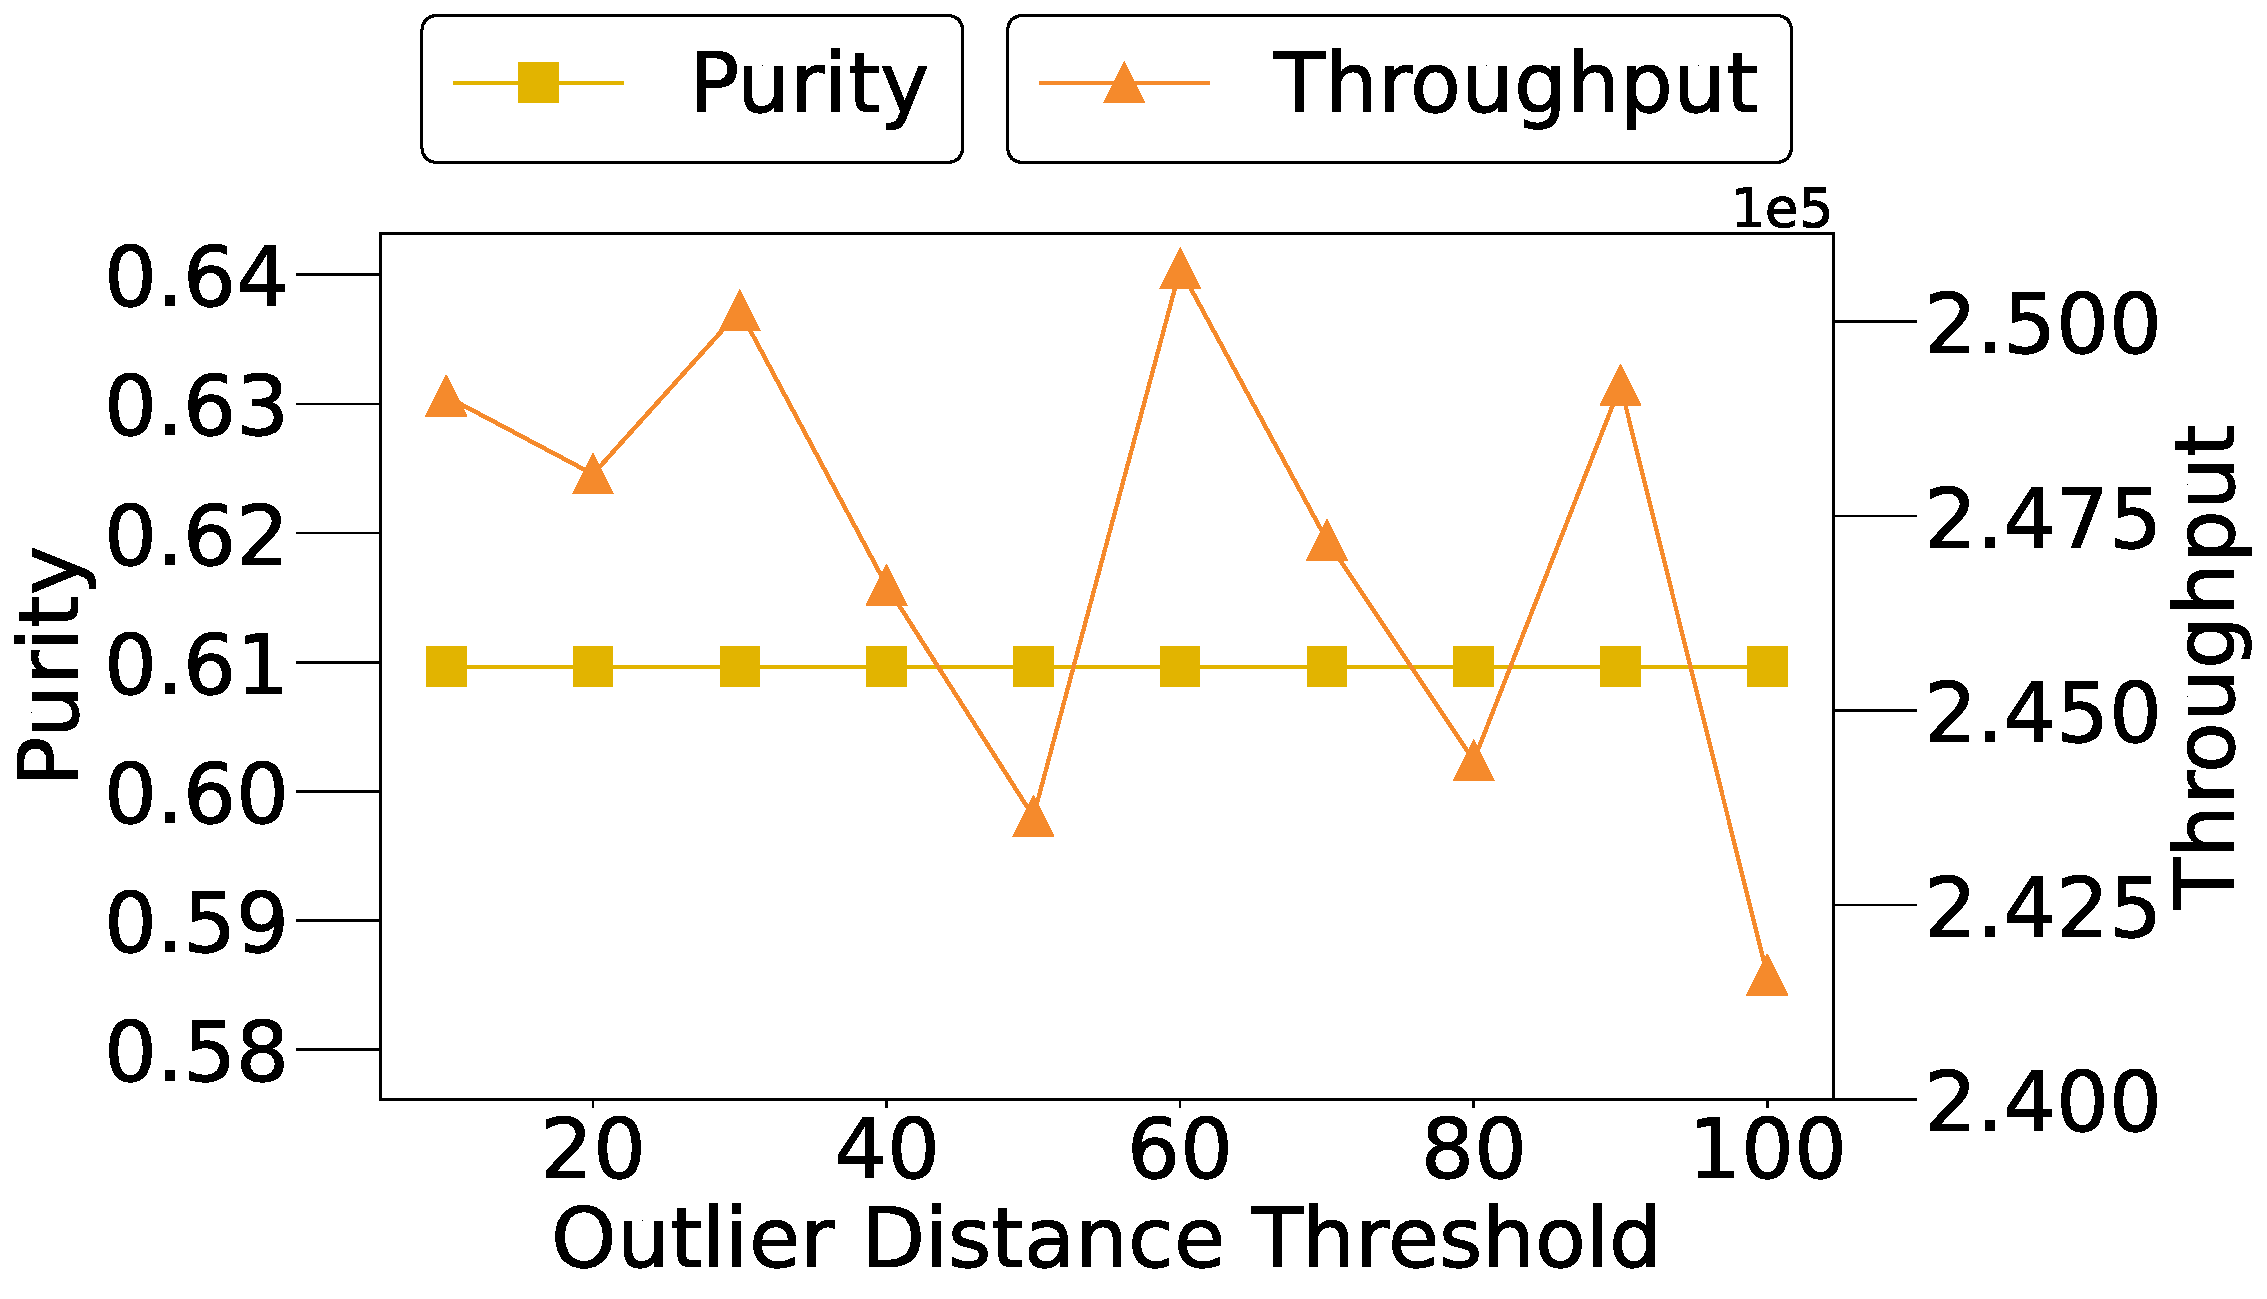
\includegraphics[width=\linewidth]{Figures/Experiment/Param/Config_Outlier_Distance_eff.pdf}
        \label{fig:outlier_distance_throughput}
	\end{subfigure}
        \centering
	\begin{subfigure}{.238\textwidth}
        \centering
        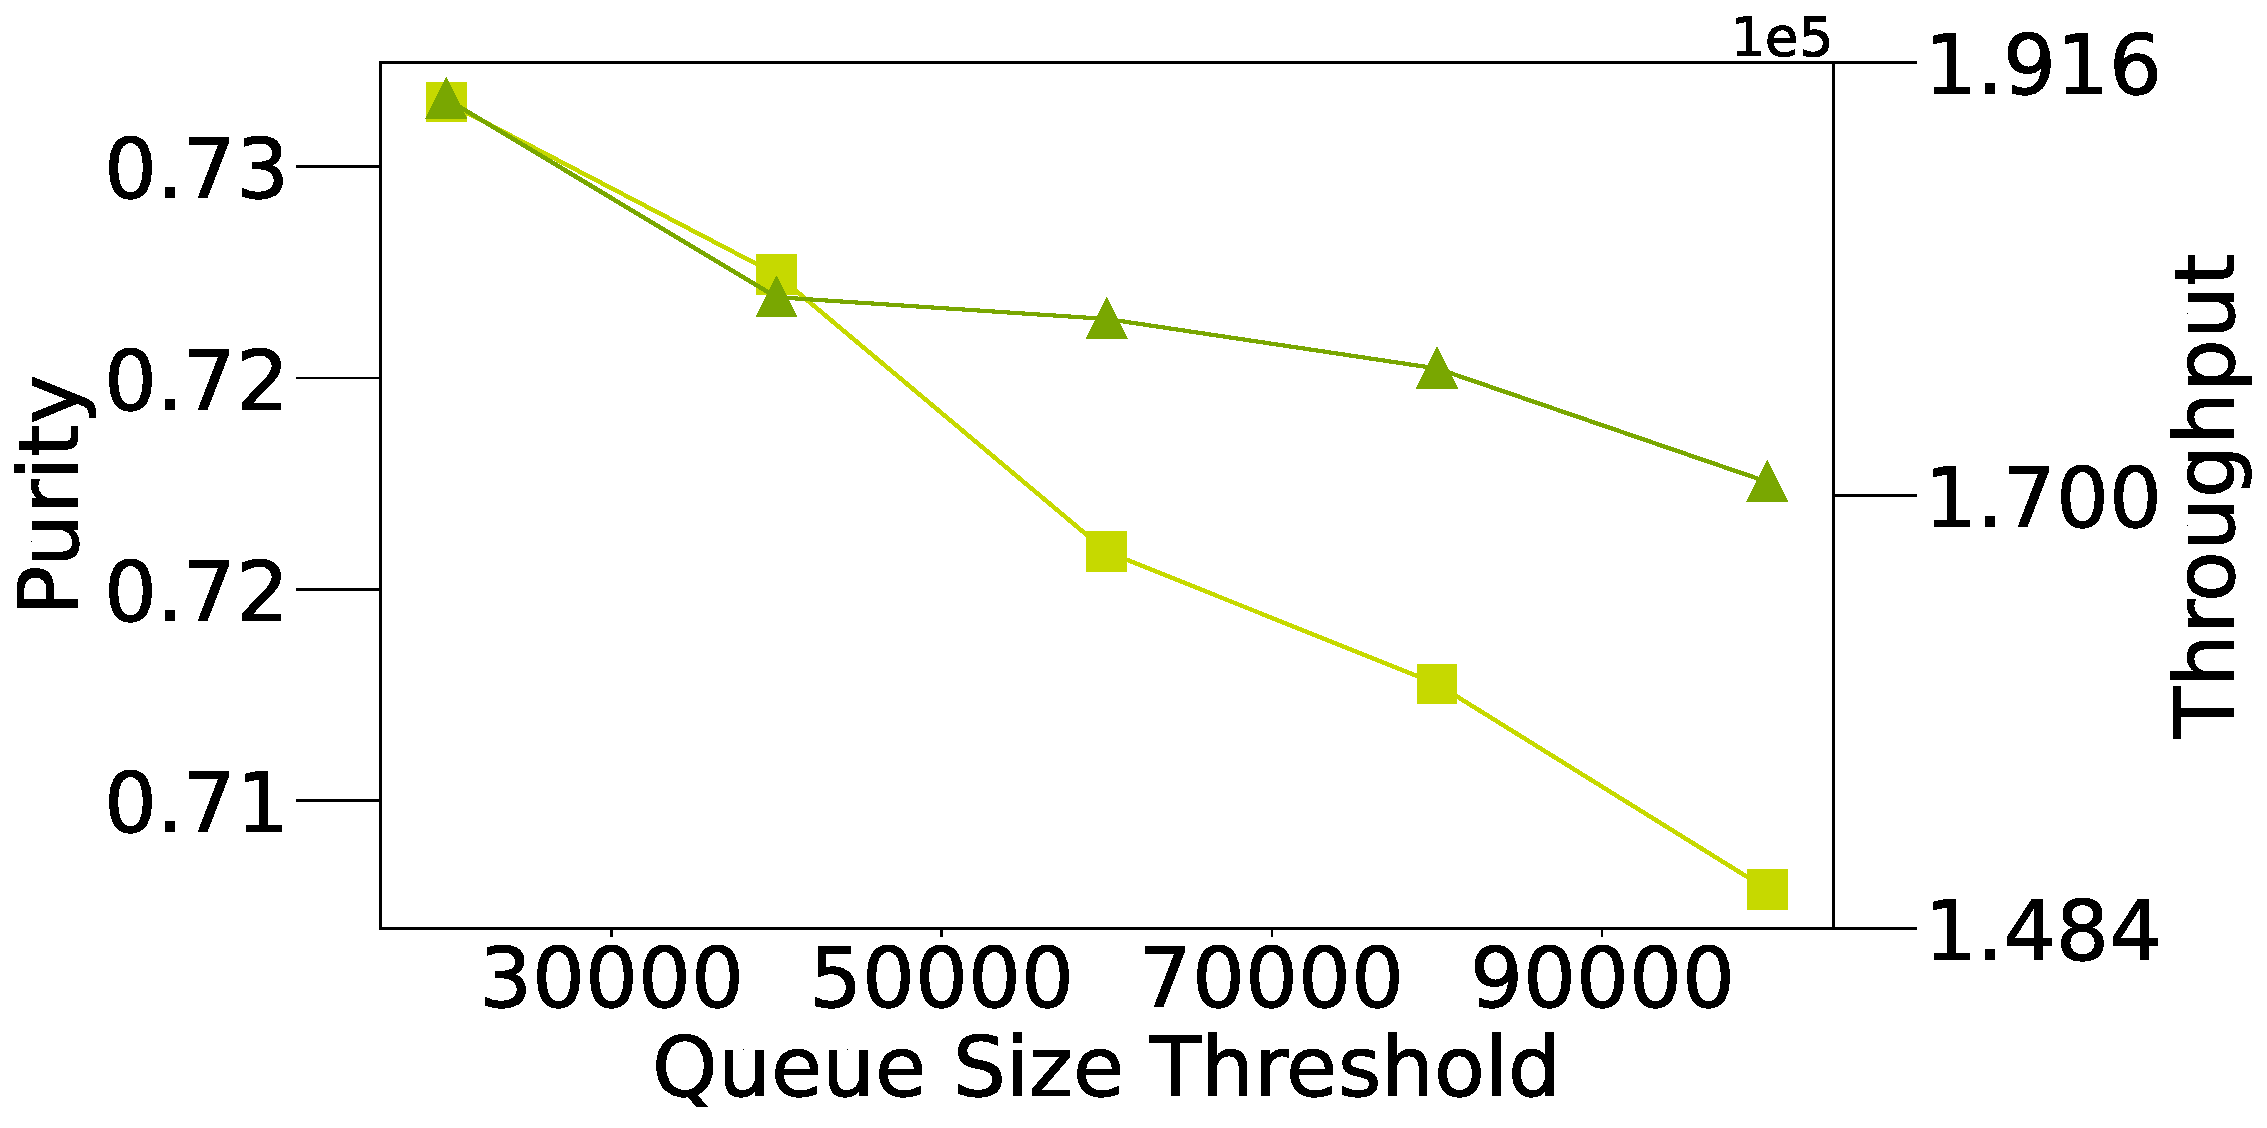
\includegraphics[width=\linewidth]{Figures/Experiment/Param/Config_Queue_Size_Acc.pdf}      
         \label{fig:queue_size_purity}
	\end{subfigure}       
  	\begin{subfigure}{.244\textwidth}
        \centering
        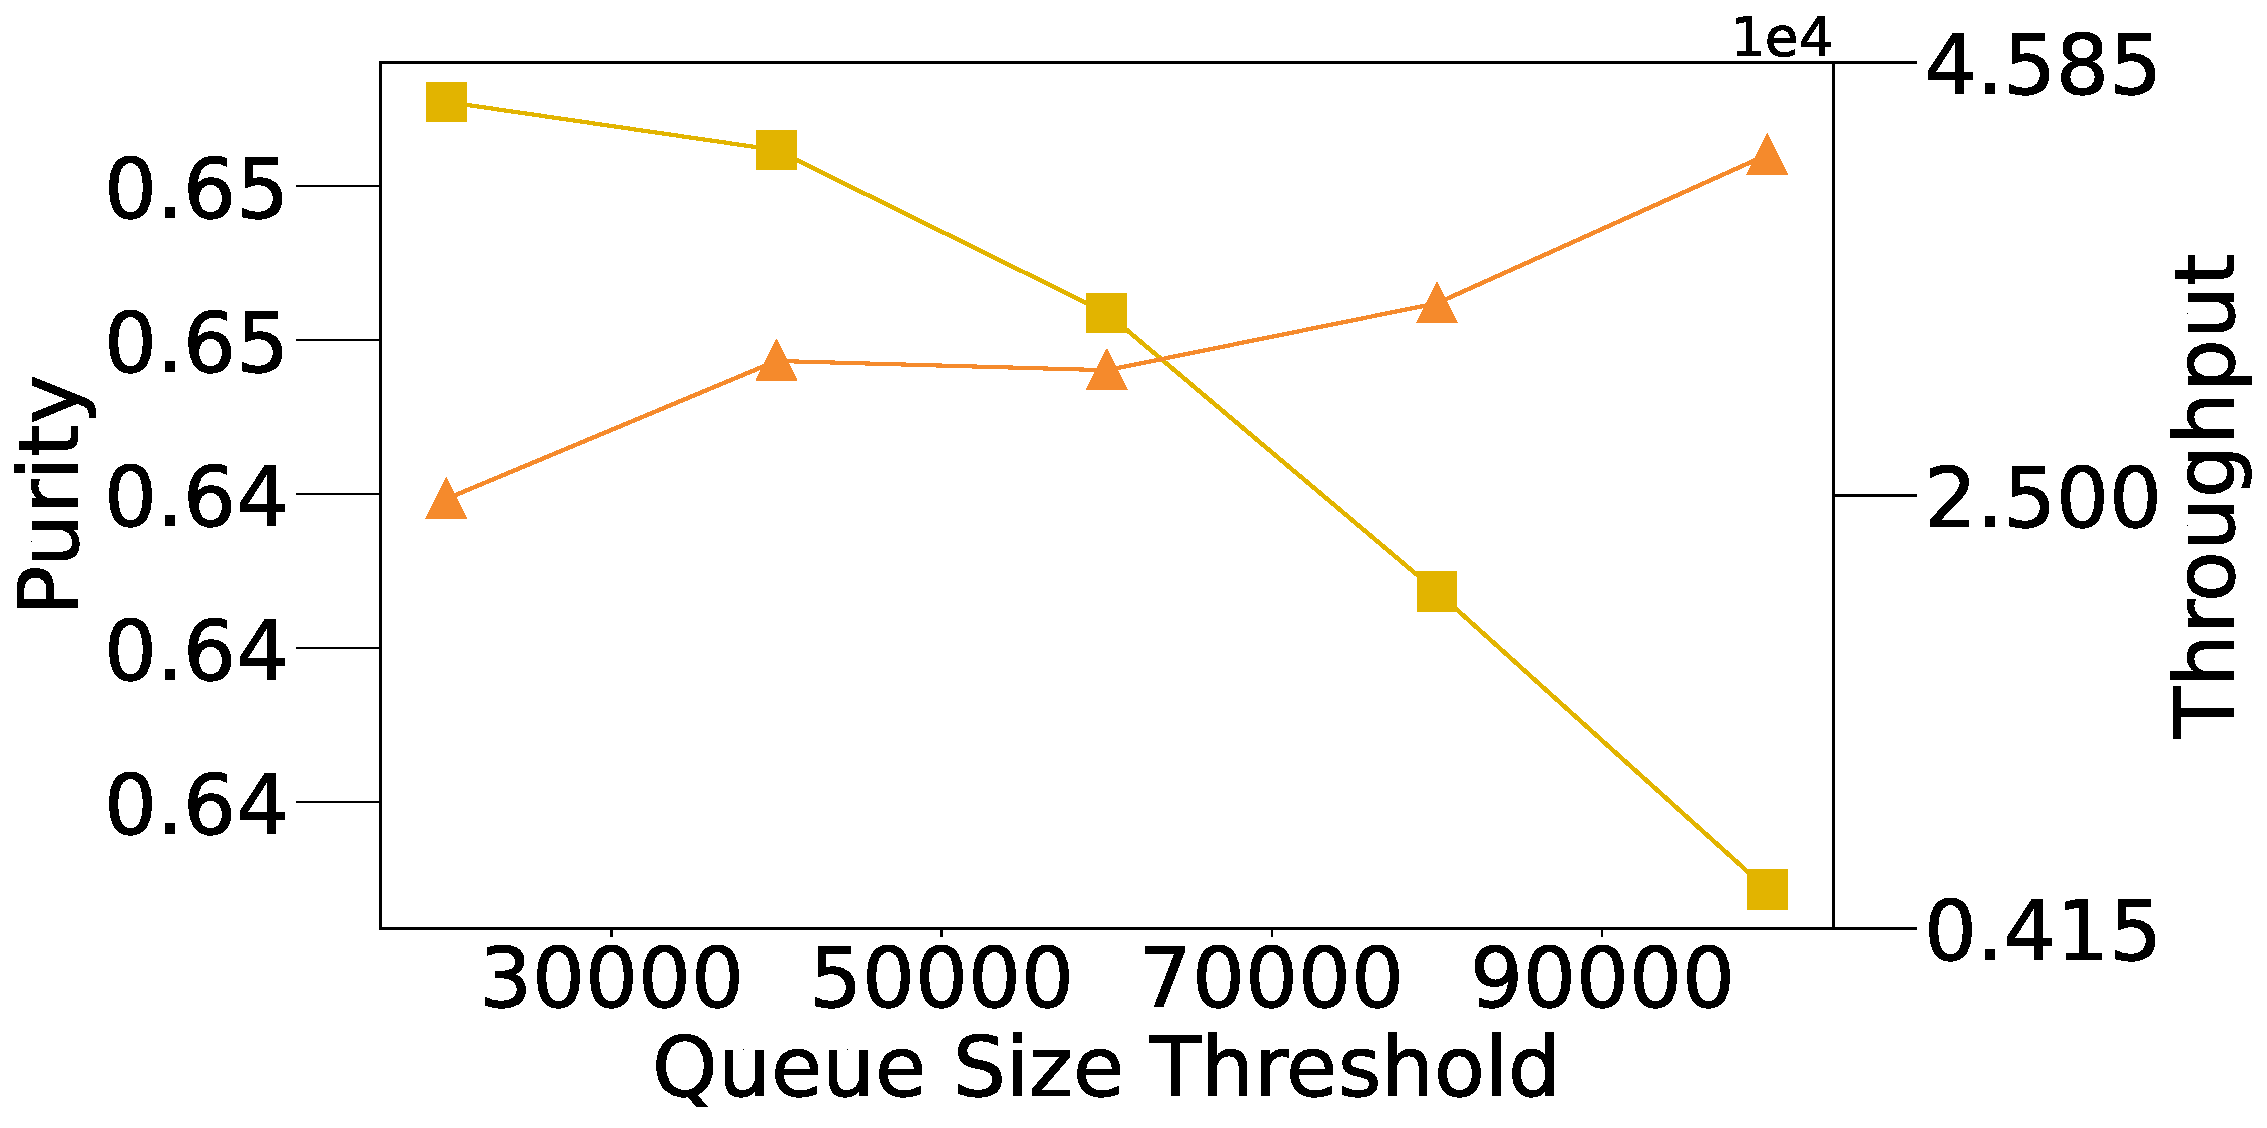
\includegraphics[width=\linewidth]{Figures/Experiment/Param/Config_Queue_Size_Eff.pdf}
        \label{fig:queue_size_throughput}
	\end{subfigure}     
        \centering
	\begin{subfigure}{.233\textwidth}
        \centering
        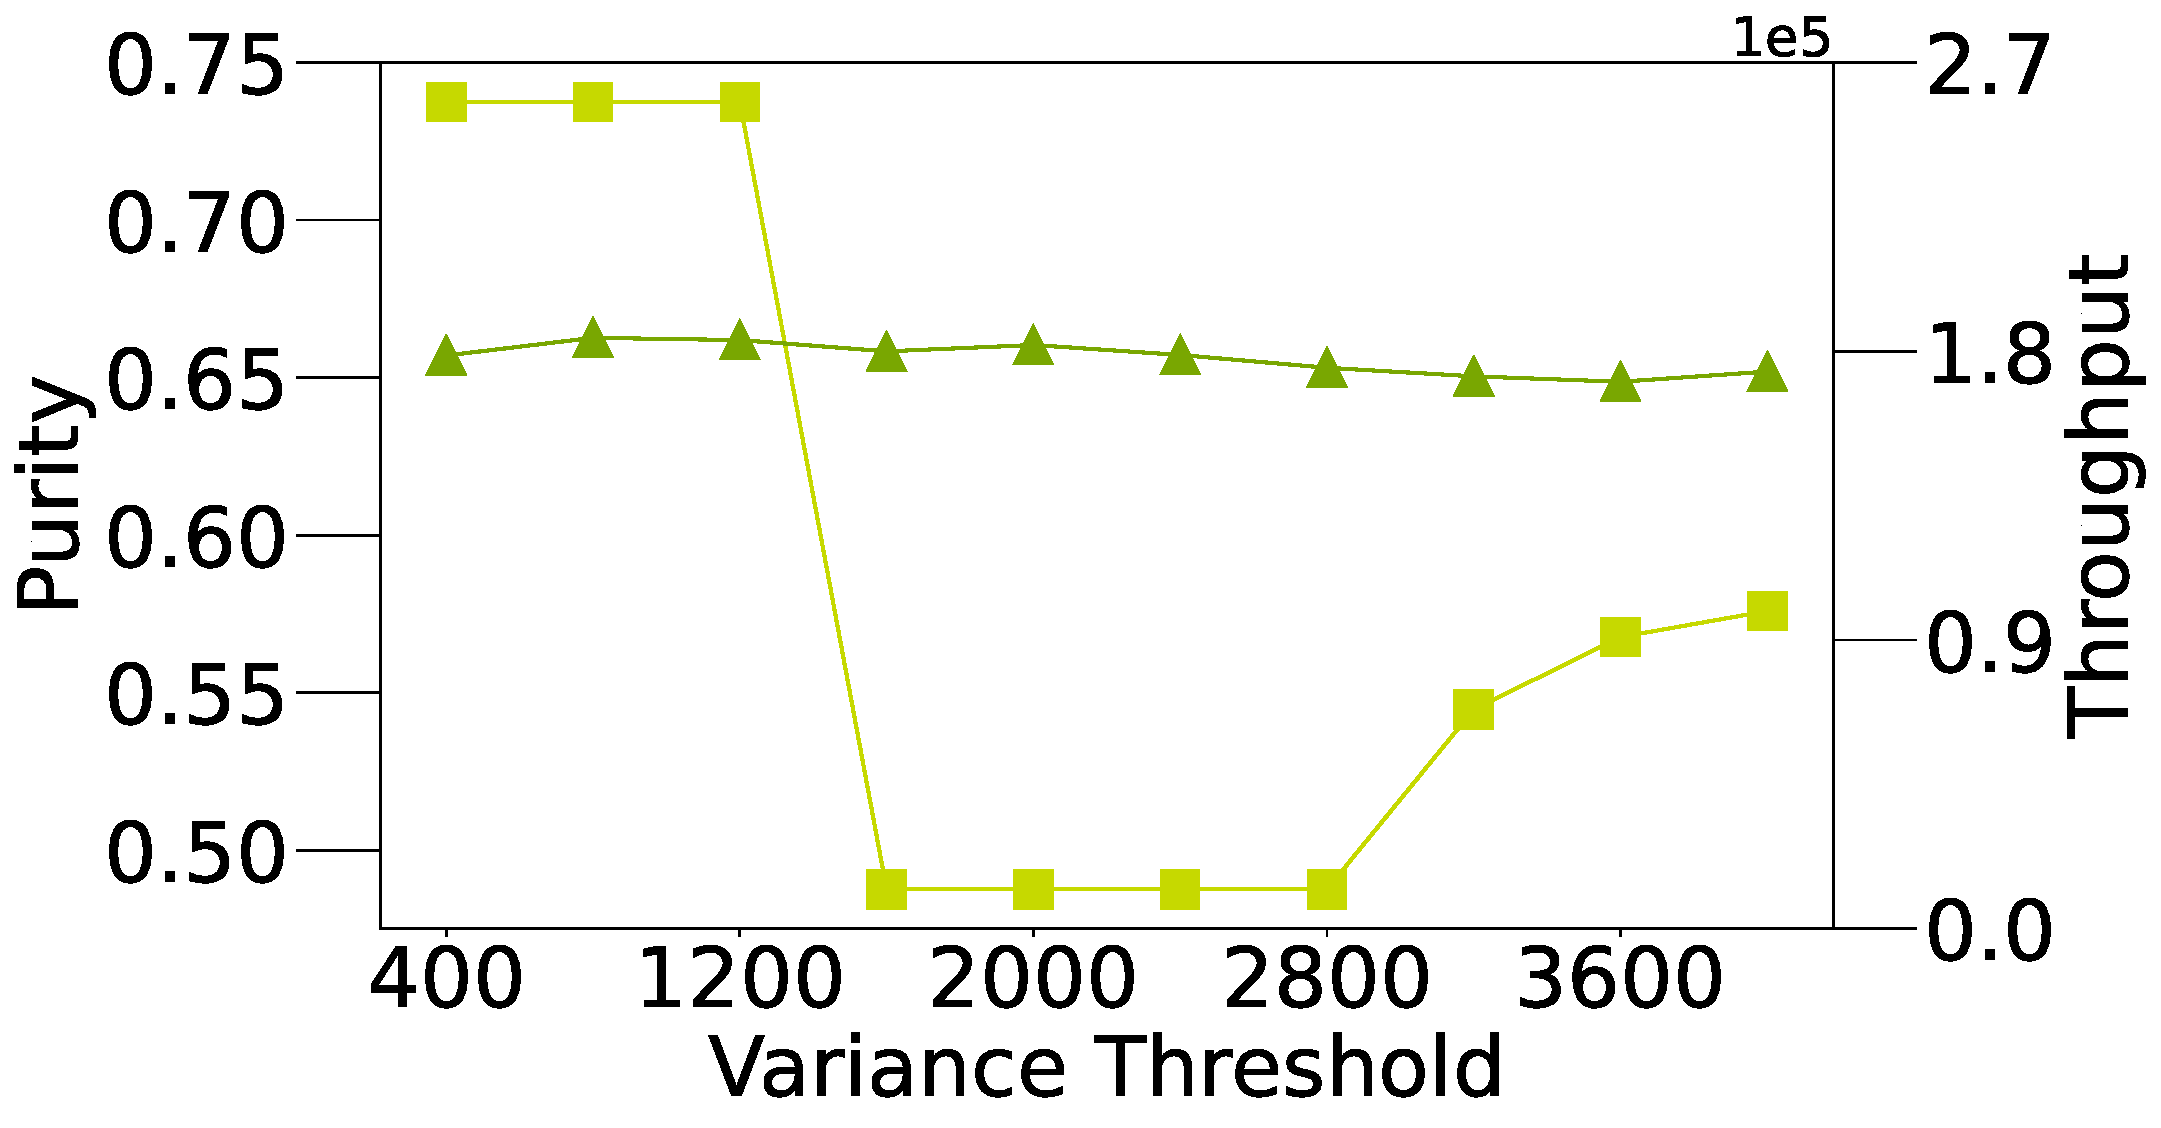
\includegraphics[width=\linewidth]{Figures/Experiment/Param/Config_Variance_Acc.pdf}      
         \caption{\algo(Accuracy)}
         \label{fig:variance_purity}
	\end{subfigure}       
  	\begin{subfigure}{.244\textwidth}
        \centering
        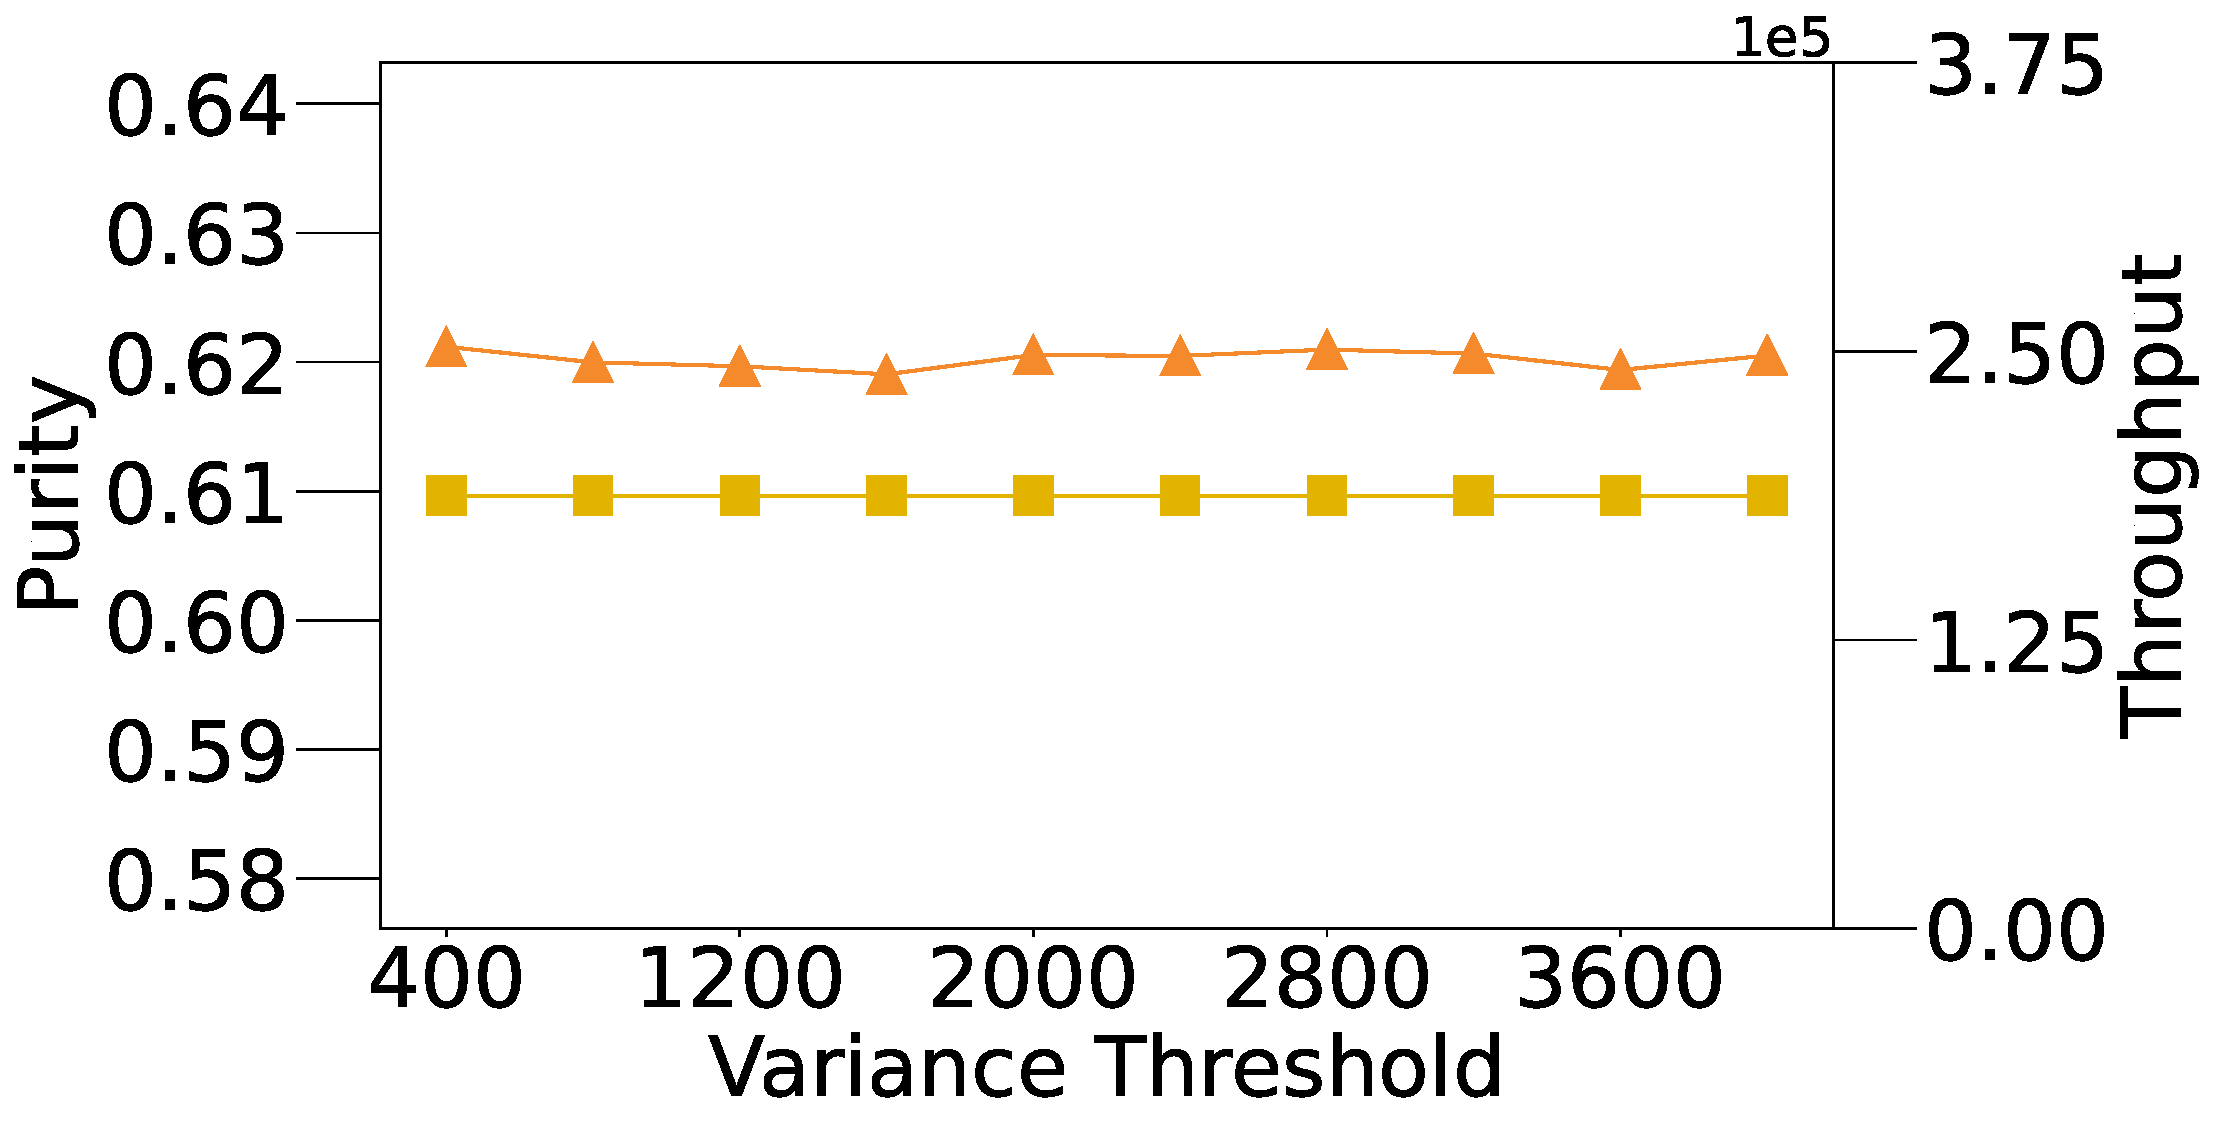
\includegraphics[width=\linewidth]{Figures/Experiment/Param/Config_Variance_Eff.pdf}
        \caption{\algo(Efficiency)}
        \label{fig:variance_throughput}
	\end{subfigure}     
    \caption{Parameter Analysis of \algo variants on \fct.}
    \label{fig:parameter_analysis}
\end{figure}